\chapter{Surface Event Modeling and Pulse Shape Simulations}

\section{Introduction}
The events on passivated surfaces create a unique modeling challenge in HPGe detectors. These interactions are best illustrated with alphas, since they deposit energy over short distances on the surface, creating large charge clouds with complex drift and collection processes, making it quite challenging to understand. We therefore study the events in terms of alpha interactions, but the same techniques can be applied to simulations of other passivated surface backgrounds such as beta and low-energy gamma interactions. This chapter begins by reviewing alpha backgrounds, then discusses the challenges in modeling surface backgrounds, and introduces a new model to address these challenges.


\section{Properties of Alpha Interactions}
Alpha particles are composed of two protons and two neutrons tightly bound together. They are identical to ionized Helium atoms with a charge of $+2$ e. The energies of alpha particles are correlated with the half-life of the parent isotope, such that the ones with the highest energies are from parent atoms with the shortest half-lives. The energies of the alpha particles are usually between about $4$ and $6$ MeV. For a given material, the linear stopping power S is defined as $-\frac{dE}{dx}$. The energy loss of charged particles in a material is then given by the Bethe formula \cite{Bethe1953}:

\begin{equation}\label{bethe_formula}
    -\frac{dE}{dx} = \frac{4\pi e^4z^2}{m_0\nu^2}NB
\end{equation}

\noindent
such that

\begin{equation}\label{bethe_B}
    \text{B}=Z\left[ \text{ln}\frac{2m_0\nu^2}{I}-\text{ln}\right(1-\frac{\nu^2}{c^2}\left)-\frac{\nu^2}{c^2}\right]
\end{equation}
\noindent
Here $\nu$ and $ze$ are the charges of the given particle. N and Z are the number density and atomic number of the absorber atoms, and m$_0$ and e are the rest mass and charge of the electron, respectively. Parameter I represents the average excitation and ionization potential of the absorber and is normally determined experimentally. 

Equation \ref{bethe_formula} suggests that the energy loss for non-relativistic particles is proportional to $1/\nu^2$, or the kinetic energy. Hence, the slower the velocity, the longer the particles spend in the vicinity of electrons of the material's atoms, and the higher the energy loss. Equation \ref{bethe_formula} is proportional to z$^2$ for a constant velocity. Thus, the heavier particles will have more energy loss for a given velocity. This results in alphas having a very low penetration depth, usually around $10$ micrometers.

The energy loss of the alpha particles can be best understood by plotting the specific energy loss along the track. The plot known as the Bragg curve is shown in figure \ref{bragg_curve_fig}. During most of the track, the energy loss increases roughly as $1$/E, as predicted by equation \ref{bethe_formula}. As the particles slow down, electron pickup reduces the charge and the curve falls off. As a result, alpha deposits a large amount of energy in a very localized area. For Germanium, this penetration depth of alpha particles is about $17.6$ - $20.0$ microns \cite{knoll_2010}. The n+ electrode is too thick for the alphas to penetrate and deposit energy. The p+ electrode in LEGEND detectors does have alpha events, but the charge collection is well understood, as the events are collected immediately and thus can be rejected easily using PSD techniques. Between these contacts is a thin insulating passivated surface, where alphas can penetrate the active volume of the detector, and the charge collection is more complex. The modeling technique developed here is focused on this surface.

\begin{figure}
\centering
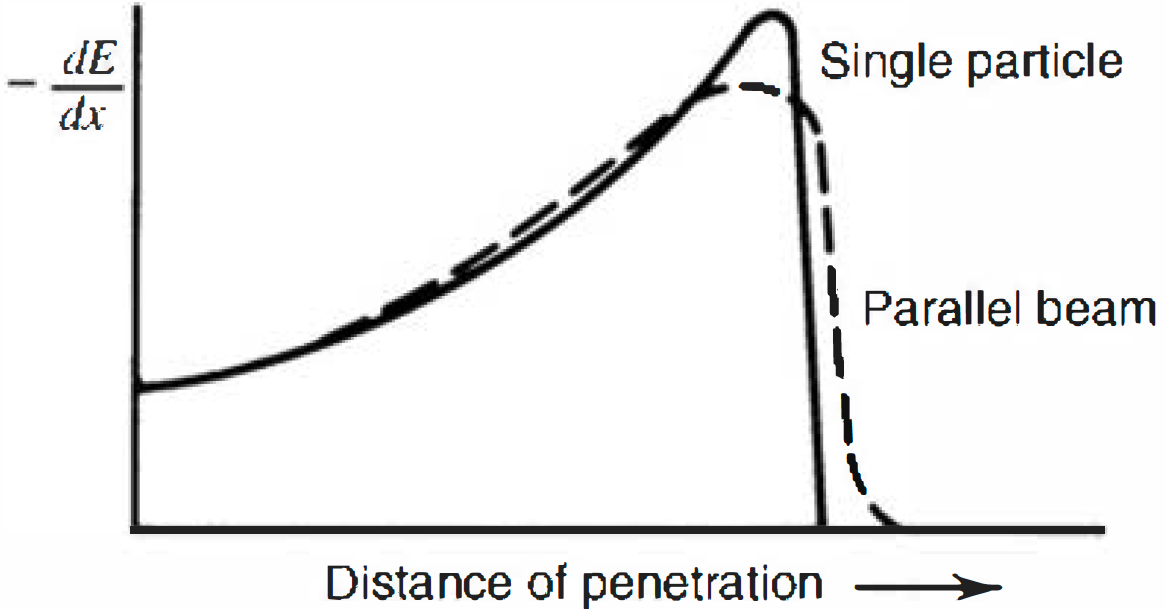
\includegraphics[width=0.5\linewidth]{ch3/figs/bragg_curve.png}
\caption{The specific energy loss in a material for an alpha particle with several MeV initial energy. Plots are shown for a single alpha particle track and for the average behavior of a parallel beam of alpha particles. Alphas lose most of their energies in a small region. Picture from \cite{knoll_2010}}. 
\label{bragg_curve_fig}
\end{figure}

\section{Alpha Background Observations}
\label{ch3_sec_alpha}
The alpha background can vary between different detector environments and experiments. The {\MJD} and {\Gerda} experiments had different spectral shapes for alpha backgrounds. In the {\MJD}, alpha events degraded more substantially in the {\onbb} ROI, while in \Gerda, prominent peaks of the $^{210}$ Po and the $^{226}$ Ra chains were identified above $5$ MeV, along with lower energy tails of partially collected surface alphas. Factors such as the cryostat environment, detector geometry, and material purity can contribute to the alpha background at Q$_{\beta\beta}$.

This can also be seen in dedicated test stands that were developed to study alpha backgrounds. Two scanning systems were developed to study alpha interactions in HPGe detectors: TUBE \cite{TUBE_paper} and GALATEA \cite{galatea_paper}. These scanners yielded conflicting dependencies of the energy loss as a function of radial position. TUBE reported that the energy degraded inversely with the detector radius, whereas GALATEA reported the opposite trend. Figure \ref{fig:dcr_waveform} shows a known alpha waveform in the TUBE data. The alpha waveform, being close to the surface, has a much sharper rise than the bulk waveform. However, the tail of the alpha waveform has an upward slope towards the end. This is due to slow collection of charges on the passivated surface. We call this effect the Delayed Charge Recovery Effect (DCR) \cite{Gruszko:2017kfx}. This feature and others like it are used to tag and reject alphas. Such cuts have been highly effective, but it is difficult to know which events are not tagged without modeling the signal.

Figure \ref{ch3_fig_L200_surface_background} shows the {\Ltwo} physics spectrum. Muon and multiplicity cuts remove backgrounds such as muons and gamma rays, and the events left are primarily surface events shown by the unfilled histogram. As shown in green, Pulse Shape Discrimination (PSD) cuts are highly effective in removing these backgrounds, but the efficiency of those cuts cannot be determined due to the lack of a model for surface events. 

\begin{figure}[!htb]
\centering
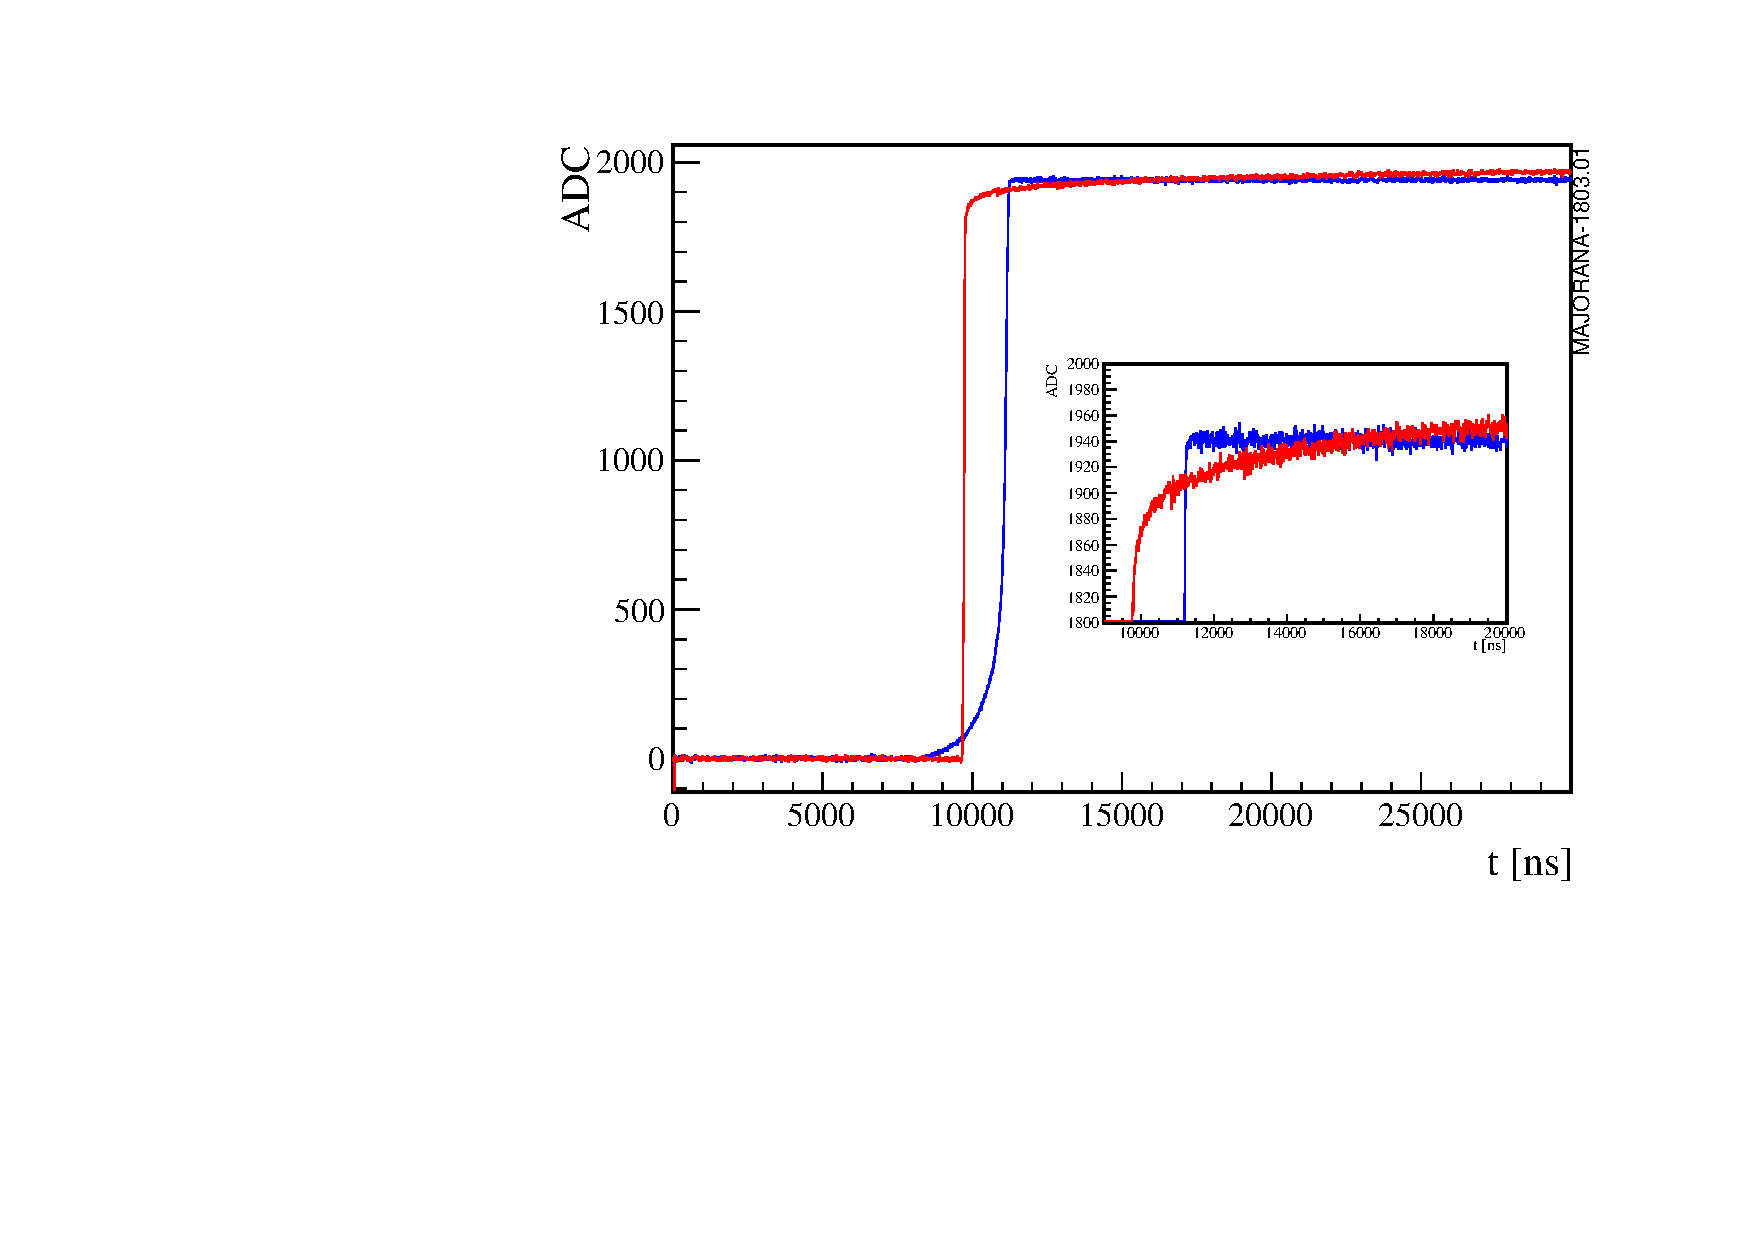
\includegraphics[width=0.9\linewidth]{ch3/figs/dcr_waveform.pdf}
\caption{An alpha waveform (red) compared to a bulk waveform (blue) in the MJD PPC detector. The DCR effect results in a slow charge collection after the fast rise of the signal, as shown by the insert plot in the box.\cite{TUBE_paper}}
\label{fig:dcr_waveform}
\end{figure}

\begin{figure}[!htb]
\centering
  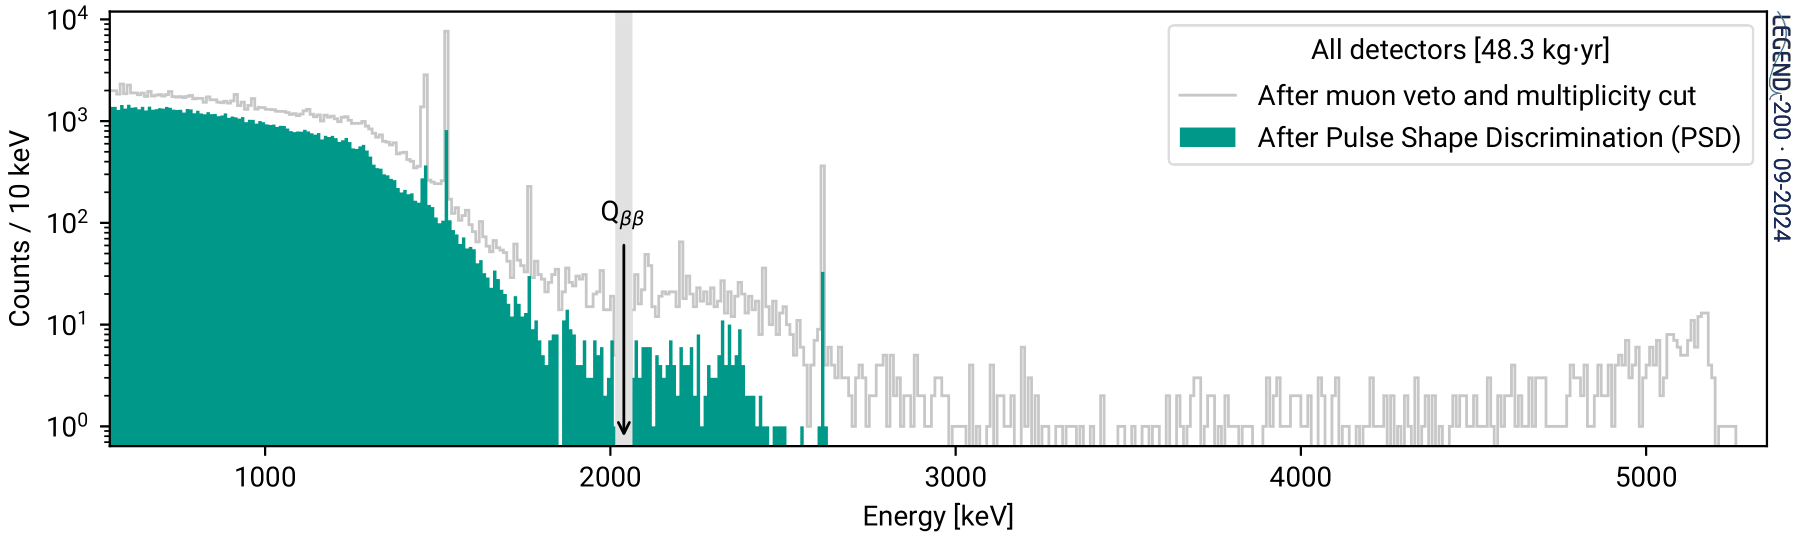
\includegraphics[width=0.99\linewidth]{ch3/figs/l200-phy-spectrum-psd.png}
  \caption{{\Ltwo} physics spectrum. The events above 3000 keV after the muon and multiplicity cut are primarily alphas. These events can be effectively removed using PSD cuts as shown in green. Credit: LEGEND collaboration}
\label{ch3_fig_L200_surface_background}
\end{figure}


\section{Challenges in Modeling Surface Events}
An alpha particle deposits an energy of approximately $4$ - $6$ MeV with a penetration depth of approximately $17.6$ - $20.0$ microns on the passivated surface. This creates a lot of charge carriers and produces a dense charge cloud. In such cases, effects such as diffusion of the charges and self-repulsion among charges become significant. These effects could also push the charge onto the passivated surface. 

The charges on the passivated surface move at slower speeds than in the detector bulk. This is mainly due to additional scattering mechanisms and modified band structure on the surface, described in \cite{MULLOWNEY201233}. In bulk, the hole and electron transport velocities can be approximated using a simple warped-band approximation. However, on the passivated surface, the band structure is altered by electrical fields normal to that on the surface. This leads to a higher probability of scattering of charges and surface-related effects such as roughness scattering.  Simulations in Ref. \cite{MULLOWNEY201233} estimate that the drift speed on the surface is $40$ to $50$ times slower than in the bulk. 

Alpha events create a highly localized, dense charge cloud close to the surface. Because the charge that ends up on the surface drifts slower than the bulk, it could get stretched into a non-spherical cloud. Thus, spherical charge cloud approximation cannot be used for such events.

%This charge cloud is difficult to model using existing simulations like {\siggen} as it uses a spherical charge approximation.


\section{Surface Charge Effect}
In operation, the HPGe detectors can accumulate static charge on the passivated surface, which affects the charge collection for surface events. The sign and magnitude of the accumulated charges can vary depending on the operating conditions. Figure \ref{ch3_fig_surface_field_sc0} shows how the presence of a surface charge alters the electric field close to the passivated surface. When there is no surface charge (top), the field lines are parallel to the surface. The presence of a negative surface charge (middle) attracts the field lines towards the surface. The positive surface charge (bottom) repels the field lines from the surface. The negative surface charge can pull the holes to the surface, where they can drift slowly. Similarly, positive surface charges can pull the electrons to the surface.

\begin{figure}
\centering
%[trim={left bottom right top},clip]
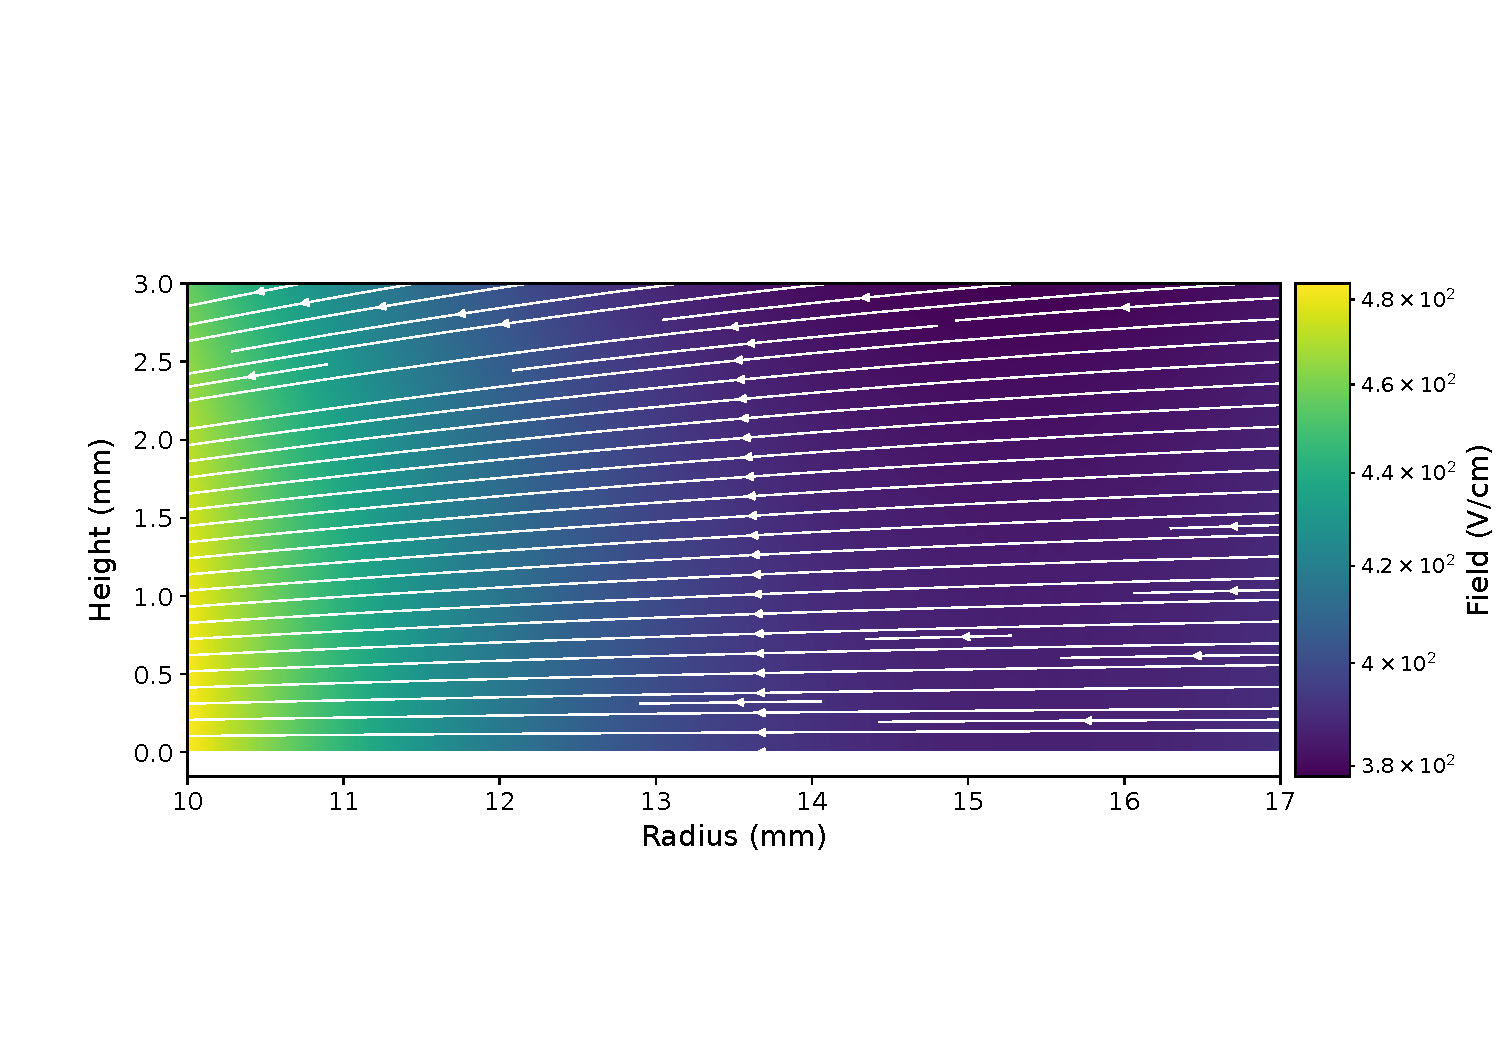
\includegraphics[trim={1.5cm 3.2cm 0.10cm 4.6cm},clip,width=0.95\linewidth]{ch3/figs/elect_field_lines_surface_ponama_1_sc_0.0.pdf}
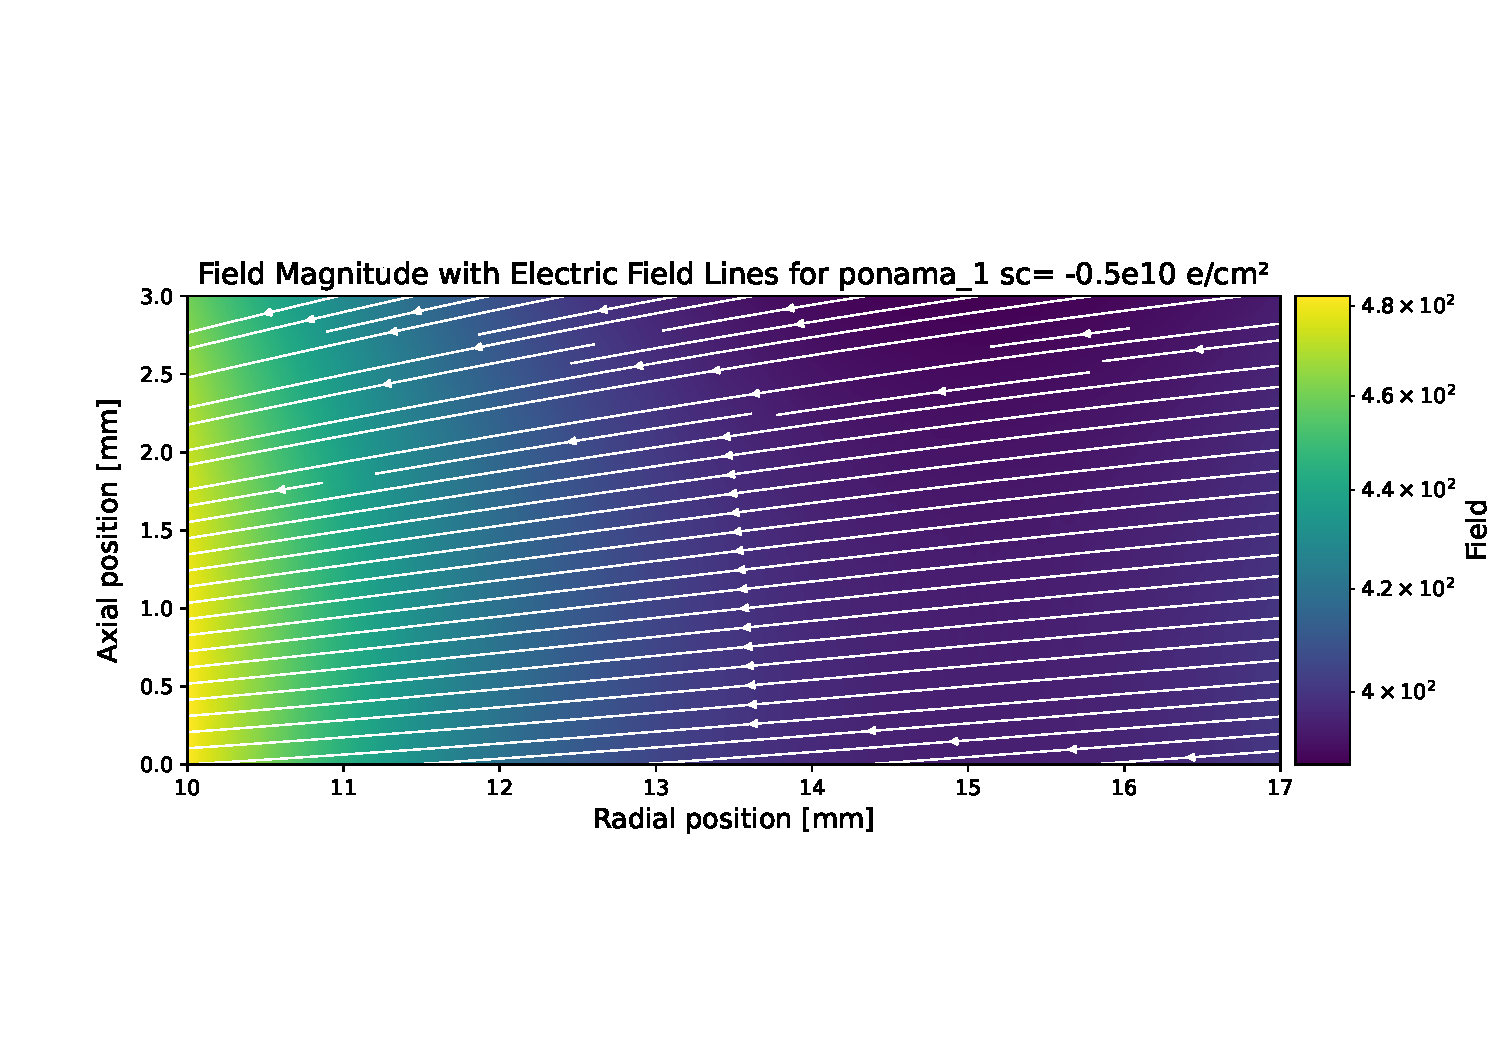
\includegraphics[trim={1.5cm 3.2cm 0.1cm 4.6cm},clip,width=0.95\linewidth]{ch3/figs/elect_field_lines_surface_ponama_1_sc_-0.5.pdf}
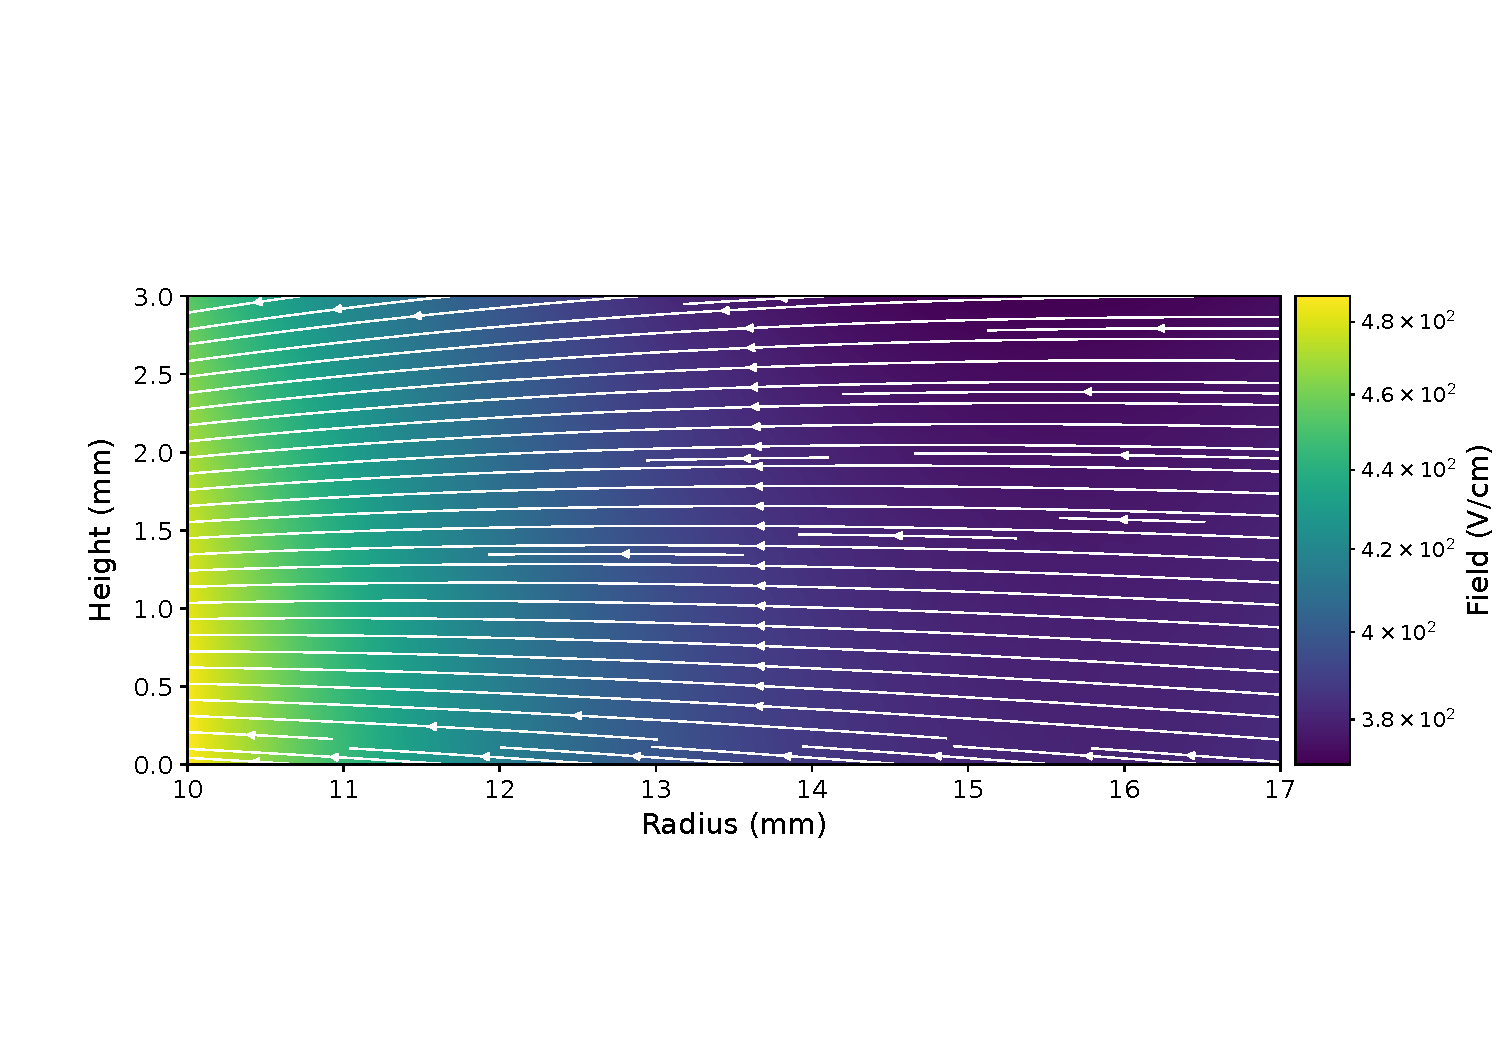
\includegraphics[trim={1.5cm 3.2cm 0.1cm 4.6cm},clip,width=0.95\linewidth]{ch3/figs/elect_field_lines_surface_ponama_1_sc_0.5.pdf}
\caption{Electric field magnitude and field lines in a region near the passivated surface of the {\ponama} PPC detector with different surface charges. The white arrows shows the direction of electric field lines. Geometry information for the detector can be found in table \ref{ch5_5_tab_ponama1_geometry}. Charges on the passivated surface can pull electrons and holes to the surface and cause energy loss and slow charge collection. Top figure has no surface charge and the field lines are parallel to surface. Middle figure has a surface charge of $-0.5 \times$ {\scunit} which pulls the filed lines to the surface. Bottom figure has surface charge of $0.5 \times$ {\scunit} that repels the field lines form the surface.}
\label{ch3_fig_surface_field_sc0}
\end{figure}

Since the surface charge changes the overall electric field of the detector, it could also alter the depletion voltage for the detector. Figure \ref{ch3_fig_deplection_sc} shows how the depletion voltage of a LEGEND PPC detector changes with surface charge. Typically, the detector's operational voltage is higher than the depletion voltage, but if the surface charges are not properly accounted for, a detector could become undepleted after being deployed in the experiment.

\begin{figure}[!htb]
\centering
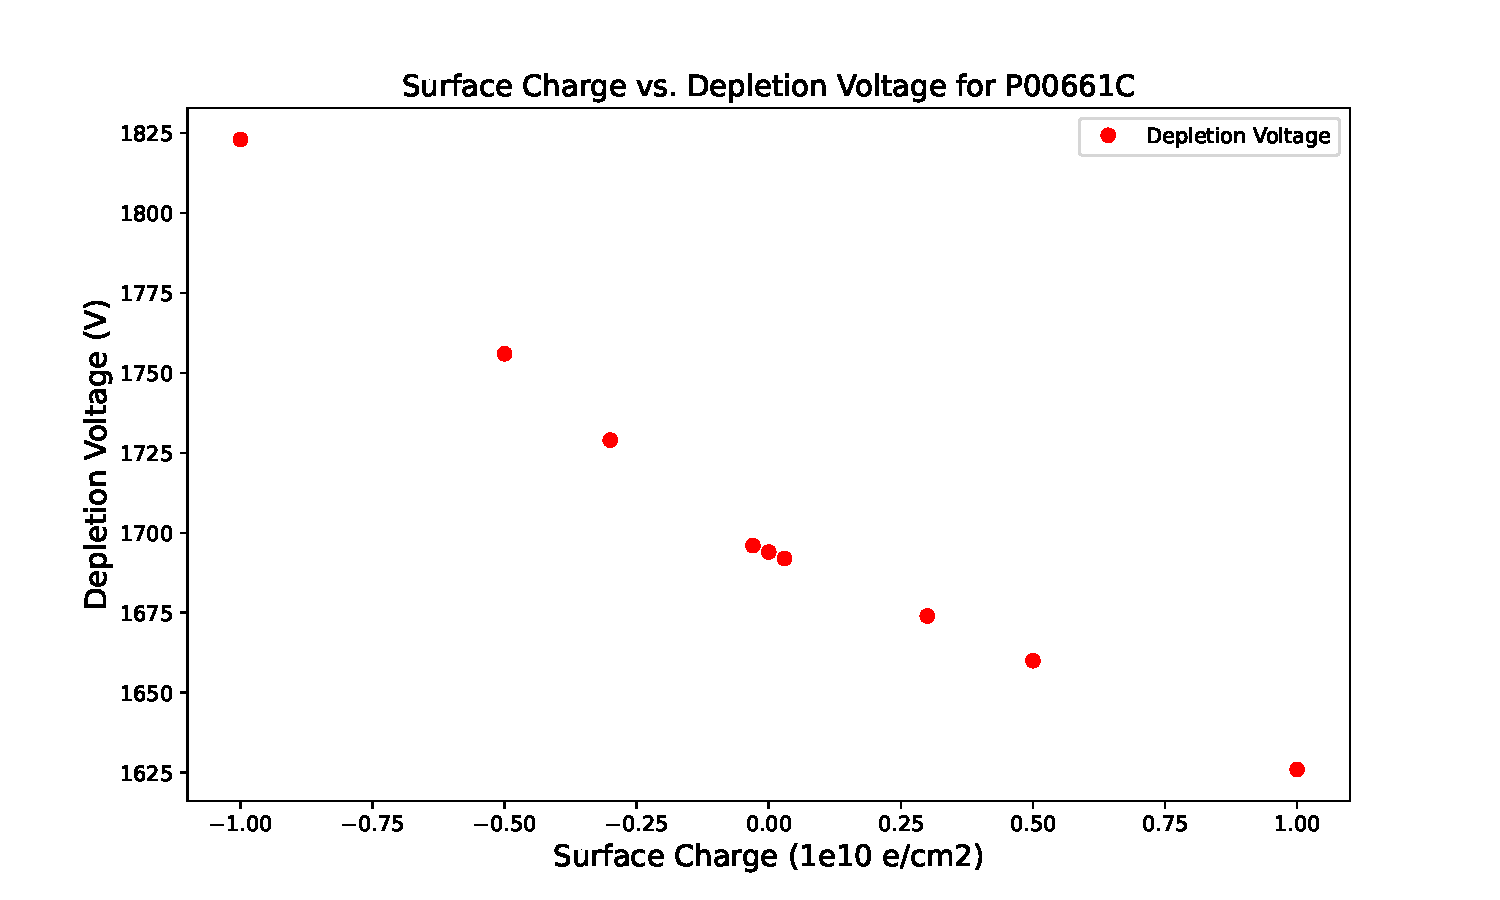
\includegraphics[trim={1cm 0.4cm 1cm 1.75cm},clip,width=0.99\linewidth]{ch3/figs/deplep_sc.pdf}
 \caption{Effect of surface charge on depletion voltage for LEGEND PPC detector P00661C. Depletion voltages calculated using {\siggen} software. The nominal depletion voltage is $1694$ V at zero surface charge. Surface charge can alter the depletion voltage and potentially cause a detector to become undepleted after being deployment.
}
\label{ch3_fig_deplection_sc}
  \end{figure}

Pulse shape simulations can help model these effects accurately and build a background model for surface events. A simulation to model surface events should allow for a non-spherical charge cloud while incorporating surface drift, diffusion, and self-repulsion. It should also properly account for surface charge effects. Next, we look at the current pulse-shape simulation frameworks that are being used by LEGEND.

\section{Current Status in Pulse Shape Simulations}
Signal formation in HPGe detectors is modeled using the Shockley-Ramo theorem. This enables the building of accurate simulations that can model the waveforms. The LEGEND Collaboration uses two HPGe signal modeling software packages, both developed in part by members of the Collaboration: {\siggen} and \texttt{SSD} simulations. 

{\siggen} is a C-based program developed by David Radford at Oak Ridge National Laboratory \cite{siggen_paper}. It consists of two components: \texttt{fieldgen} and {\siggen}. \texttt{fieldgen} is used to calculate the electric potential and weighting potential of point-contact detectors in two dimensions. {\siggen} then uses the weighting potential calculated from \texttt{fieldgen} to generate signals for a charge originating at a given point in the detector using the Shockley–Ramo theorem. \texttt{fieldgen} simulations can be used to calculate the depletion voltage, the volume of the depletion region, and the capacitance of the detector. Diffusion in {\siggen} is approximated using a Gaussian convolution, and there is no mechanism to model nonspherical charge clouds since {\siggen} uses point charges to represent the entire charge cloud. {\siggen} simulations have been crucial in the design and manufacturing of the LEGEND detectors, as they allow precise modeling of electric fields and projected PSD performance.


SolidStateDetectors.jl (\texttt{SSD}) is a software package developed by the Abt group at the Max Planck Institute in Munich \cite{Abt:2021SSD}. It is written in Julia and can perform calculations in full $3$-dimensions. \texttt{SSD} can calculate electric fields and potentials outside the detectors. The \texttt{SSD} enables full $3$-D diffusion and models self-repulsion in the signal. It does this by using a limited number of charges, each of which represents many real charges. Charges are individually tracked using their position and velocity. The electric field calculation can be performed on GPUs. 


\section{{\ehd}}
{\ehd} is a newly developed method to simulate surface events while directly simulating diffusion and self-repulsion. It is a specialized model designed to simulate passivated surface interactions. The model uses $2$-D approximations to optimize run-time while adjusting for $3$-D effects. The original software version was developed in C by David Radford and built as an extension to {\siggen}. As charges drift through the detectors, the software keeps track of charge densities at a pixel-by-pixel level, which allows for nonspherical charge clouds and for extremely large variations in charge density at different positions in the detector. The charges that end up on the surface have their velocities reduced by a predetermined factor, which is set based on dedicated computational modeling of passivated surfaces in HPGe detectors. {\ehd} also enables simulation of the effects of surface charges. The simulation is performed in the r and z directions while assuming $\phi$ symmetry; therefore, the charge cloud is simulated by a ring of charges, and the calculations account for the $3$-D effects using analytic approximations. This approach does not take into account the varying mobilities as a function of the crystal axis because this is a small effect for events dominated by surface drift.


\subsection{Charge Transport Equation}
\label{sec:charge_transport_eq}
To model the time evolution of electrons and holes in a detector, we used the continuity equation added together with drift and diffusion terms. Let $\rho(r,t)$ be the charge density of one carrier (electron or hole) at position $r$ and time $t$. The total current density, $J$, has two contributions: 

\begin{itemize}
  \item Diffusion current $-D\nabla \rho$, where $D$ is the diffusion coefficient,
  \item Drift current $\mu\,\rho\,E$, where $\mu$ is the mobility and $E$ is the electric field. 
\end{itemize}

Combining these into the continuity equation for charge conservation gives:
\begin{equation}
\label{ch3_eq_charge_transport}
\frac{\partial \rho(r,t)}{\partial t}
\;=\;
\nabla \cdot \Bigl(D\,\nabla\rho(r,t)\Bigr)
\;-\;
\nabla \cdot \Bigl(\mu\,\rho(r,t)\,{E}(r,t)\Bigr)
\end{equation}

The first term on the right-hand side describes how thermal diffusion spreads the charge carriers from regions of higher density to lower density. The second term captures the drift of  charges under the influence of the electric field. To solve this numerically in discrete time steps, we write $t^{n+1} = t^n + \Delta t$. Using a first-order approximation, we get:
\begin{equation}\label{ch3_eq_ehdrift_discrete}
\rho^{n+1}({r}) 
=
\rho^n({r})
\;+\;
\Delta t \,
\Bigl[
\nabla \cdot \bigl(D\,\nabla\rho^n({r})\bigr)
\;-\;
\nabla \cdot \bigl(\mu\,\rho^n({r})\,{E}^n({r})\bigr)
\Bigr]
\end{equation}
where $\rho^n({r})$ and ${E}^n({r})$ denote the density and electric field at
the $n$-th time step, respectively. After discretization, we update both the drift and diffusion terms in a single time step $\Delta t$. Although drift and diffusion have different characteristic timescales, we adopt the one that is more stringent. Typically, drift in an electric field changes more quickly. The time step is thus set using this assumption by calculating the Courant number, discussed in Section \ref{ch3_sec_courant}. To solve this equation, {\ehd} takes the Lagrangian splitting approach. This means that each step, such as diffusion and charge drift, is solved independently, and then the net effect is calculated by combining them. Figure \ref{fig:ehd_flowchart} shows how the {\ehd} program works. 

\subsection{Initial Setup}
During the initial setup, the detector is divided into a grid. The coordinates of this grid are shown in figure \ref{ch3_fig_coordinates}.

\begin{figure}[!htb]
\centering
%[trim={left bottom right top},clip]
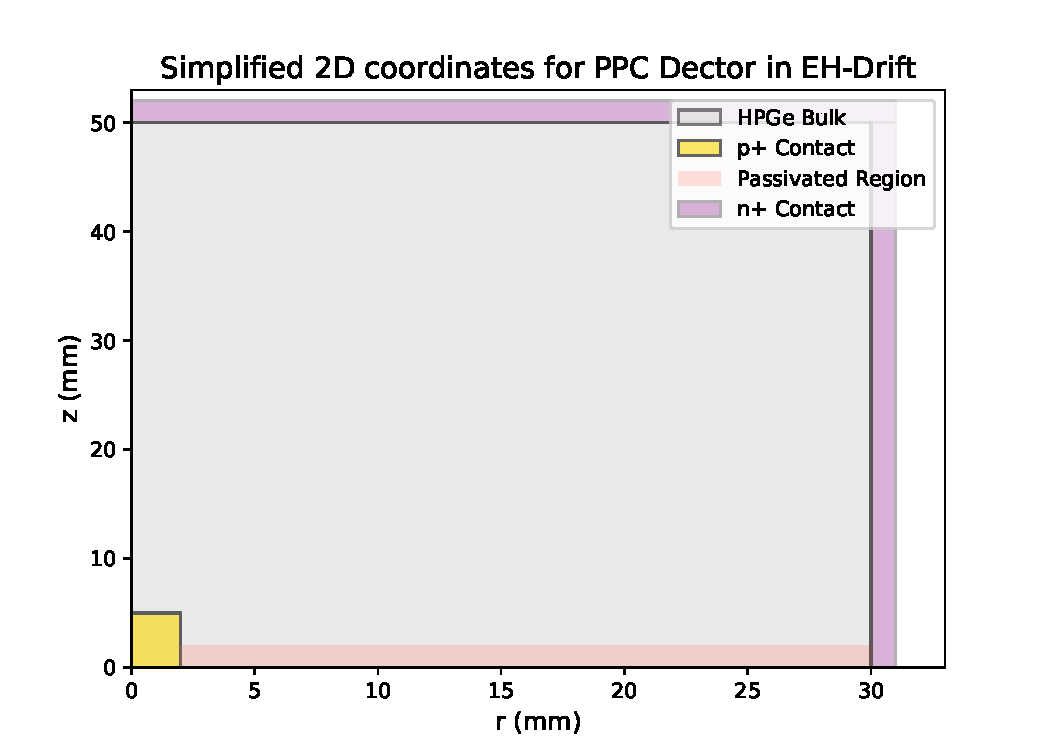
\includegraphics[width=0.9\linewidth,trim={0pc 0pc 0pc 0pc},clip]{ch3/figs/ppc_coordinates.pdf}
\caption{Diagram showing a simple setup and coordinates in {\ehd} for a PPC detector. The n$^+$ electrode is kept at high voltage while p$^+$ is kept at zero. Passivated region is the region in between the two electrodes.}
\label{ch3_fig_coordinates}
\end{figure}

Each point on the grid has a value for the potential, weighting potential, electron and hole densities, and impurity. The boundary conditions are then set according to the detector's input geometry, surface charge, and bias voltage. Next, the electric potential and weighting potential are calculated using an over-relaxation algorithm. The capacitance and depletion are estimated to understand the detector's behavior. The capacitance is calculated by relating two equations for the energy stored in an electric field:
\begin{equation}
    \frac{1}{2} C V^2 = \frac{1}{2} \epsilon \int E^2 dV
\end{equation}

\begin{equation}
    C = \frac{\epsilon \int E^2 \, dV}{V^2}
\end{equation}
where C is the capacitance of the detector, $\epsilon$ is the permittivity of the medium, E is the electric field magnitude, and V is the bias voltage. The depletion voltage is calculated by finding the minimum bias required to fully deplete the detector. Then the software checks to find local minima in the potential to help identify any pinch-off depletion region. The initial charge densities are distributed at a given location on the basis of the position, usually over two adjacent grid points. The initial densities are determined using the following:

\begin{equation}
\rho_E \Bigl(10^{10} \,\frac{\mathrm{pairs}}{\mathrm{cm^3}}\Bigr) = \rho_H  \;=\;
\frac{ \mathrm{E}\bigl(\mathrm{keV}\bigr)\ \times \bigl(1\,\mathrm{keV} = 1000\,\mathrm{eV}\bigr) \times\,10^{-10} }{\bigl(3\,\mathrm{eV/pair}\bigr)\,\times\, \bigl(10^{-3}\,\mathrm{cm}^{3} = 1\,\mathrm{mm}^3\bigr)\ \times \bigl[\text{grid}\,(\mathrm{mm})\bigr]^3 }
\label{eq:density_with_units}
\end{equation}

where $\rho$ represents the density of the charge (electrons or holes) in units of \(10^{10}/\text{cm}^3\). The energy deposited E is the energy deposited in keV, which is first converted to eV. The factor of $10^{-10}$ accounts for the final units. The approximate energy required to generate an electron-hole pair in Germanium is $3$ eV. Finally, dividing by \(\text{grid}^3\) in mm normalizes the number of charge pairs generated by the volume of the grid. The densities for both holes and electrons are deposited equally in points (z,r) and (z+1,r). The density is then multiplied by a calibration factor that is tuned such that the $2$-D simulation of the self-repulsion effect matches the $3$-D model. The calibration factor we found in dedicated studies was a factor of 20 for all detector geometries.

\begin{figure}[!htb]
\centering
%[trim={left bottom right top},clip]
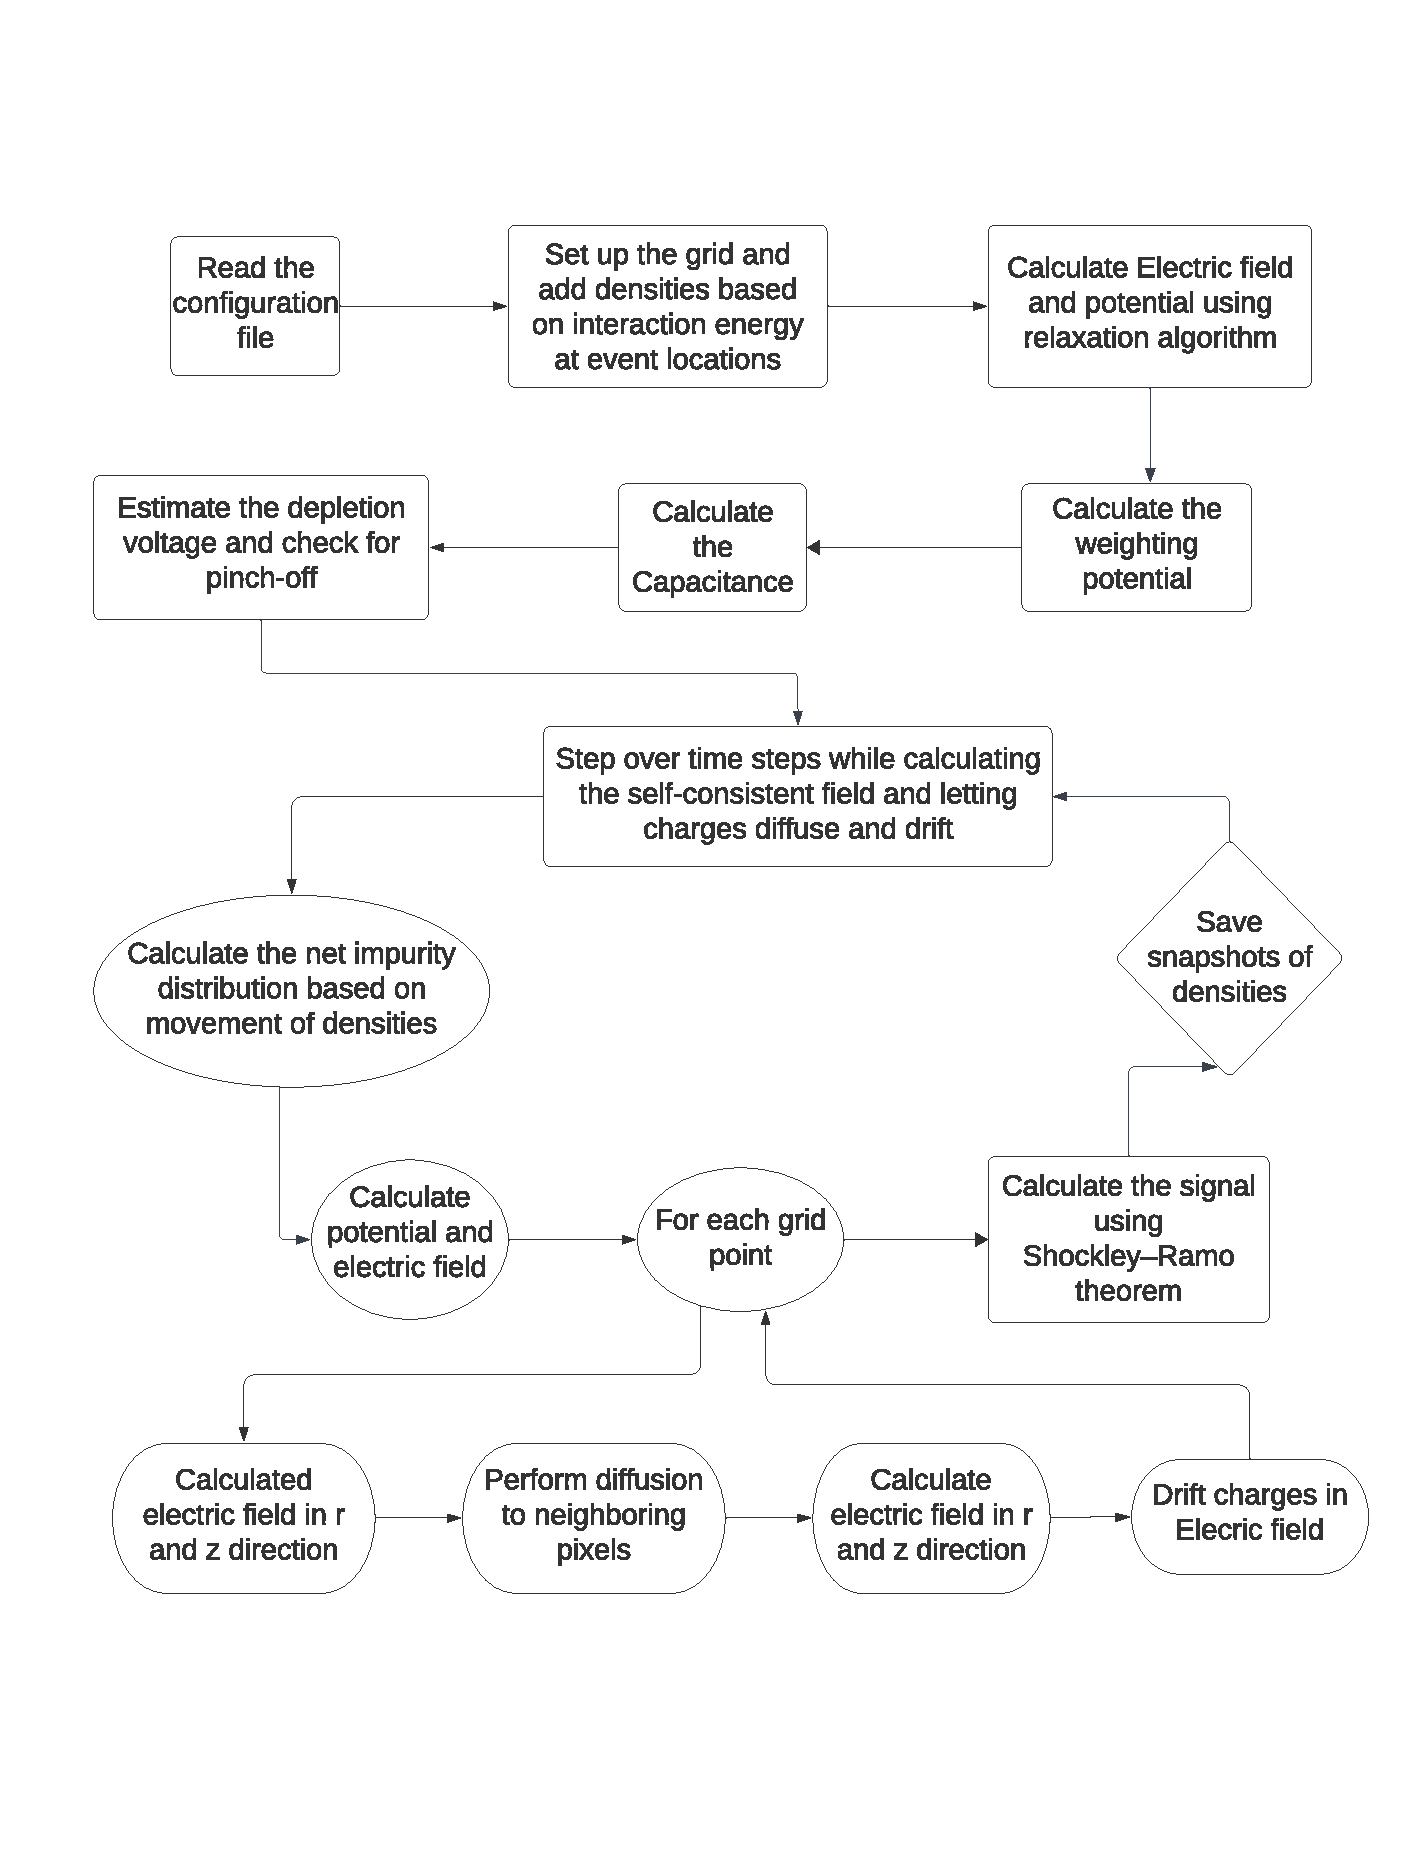
\includegraphics[width=0.99\linewidth,trim={2pc 10pc 1.5pc 9pc},clip]{ch3/figs/ehd_flowchart.pdf}
\caption{A flow chat illustration the {\ehd} steps. The initial steps to calculate intrinsic parameters of the detector (e.g. weighting potential, capacitance, etc.) are performed once. Then subsequent loops step through each time step and each grid point to track the movement of charge clouds.}
\label{fig:ehd_flowchart}
\end{figure}

After the initial setup, the program steps through a series of time steps. The charges are allowed to diffuse and then drift in the electric field created by the combination of the intrinsic detector field and the self-repulsion of charges.  The electric field is updated at each time step by solving Poisson's equation with the net charge density, including both fixed impurities and free charges, to account for effects like self-repulsion. The calculation of the electric field is discussed in Section \ref{ch4_sec_relax_algo}. In the following sections, we discuss the rest of the critical components of {\ehd}.

\subsection{Diffusion}
Diffusion arises from the random thermal motion of electrons and holes, which causes them to spread out from regions of high concentration into regions of lower concentration. In thermal equilibrium, the diffusion coefficient $D$ and the mobility $\mu$
are related by the Einstein relation:
\begin{equation}
D = \mu \frac{k_B T}{q},
\end{equation}
where $k_B$ is Boltzmann's constant, $T$ is the absolute temperature, and $q$ is the elementary charge. Thus, if the mobility $\mu$ is known or has been fitted to experimental data, $D$ can be determined for a specified temperature. In germanium at cryogenic temperatures (e.g. $\sim 77$ K), the mobilities are
sufficiently large that diffusion can still have a noticeable effect on the final spread of a charge cloud, although it is smaller than under room temperature conditions.

In {\ehd} the diffusion is simulated by redistributing the charge among neighboring grid cells in the $(r)$ and $(z)$ directions using the diffusion coefficients. During each time step $\Delta t$, a fraction of the carriers in the cell $(z,r)$ diffuse to adjacent cells $(z\pm1,\,r\pm1)$ according to two quantities: $\delta_z$ and $\delta_r$. These fractions are computed from an approximate diffusion parameter $f$ and the local drift velocity magnitudes $\lvert \mathbf{v_z} \rvert$, $\lvert \mathbf{v_r} \rvert$ as follows:
\begin{align}
   \delta_z &\;=\; \frac{\Delta x \;\,v_z \;f}{E_z}\label{eq:deltaez}\\
   \delta_r &\;=\; \frac{\Delta x \;\,v_r \;f}{E_r} \label{eq:deltaer}
\end{align}
where $\Delta x$ is the grid size, $v_{z}$ and $v_{r}$ are the drift velocities, $E_{z}$ and $E_{r}$ are the local field components, and $f$ incorporates the diffusion coefficient $D$ and corrections for grid sizes. If $E_z$ or $E_r$ is below $1\,\mathrm{V/cm}$, the program sets $\delta_z = 0$ or $\delta_r=0$ assuming that the low field regions produce negligible drift velocity.

\subsubsection*{Volume Correction}
In cylindrical coordinates $(r,z)$, each radial ring has a different physical area. The simulation tracks these scaling factors with arrays:
\[
\texttt{s1}[r] = 1 + \frac{0.5}{r-1}, 
\qquad
\texttt{s2}[r] = 1 - \frac{0.5}{r-1},
\] 
For r=$1$ and r=$0$, the code uses a special fixed weighting factor to handle the geometry. These scalars adjust the amount of charge that is diffusing into or out of the neighboring ring. Specifically, if $\delta_r$ is the fraction of carriers leaving cell $(r)$ in
the $+r$ direction, the actual increase in the neighbor cell
$(r+1)$ is multiplied by $\texttt{s1}[r]$, while the old cell is
reduced by the same fraction multiplied by $\texttt{s1}[r]$ to
balance volume differences. Similarly, diffusion to cell $(r-1)$ 
uses $\texttt{s2}[r]$. The same volume correction is used in the field calculation.

\subsubsection*{Diffusion Density Update}
After computing the diffusion fractions $\delta_z$ and $\delta_r$, the code subtracts those amounts from the point's density and adds them to the four neighbors:
\begin{align}
  \rho^{\mathrm{new}}(z,\,r+1) &\;\mathrel{+}= \;\rho^{\mathrm{old}}(z,\,r)\times\delta_r \times s_1(r) \times \frac{r-1}{r} \label{ch3:eq:diffusion_update_1} \\
  \rho^{\mathrm{new}}(z-1,\,r) &\;\mathrel{+}= \;\rho^{\mathrm{old}}(z,\,r)\times\delta_z \label{ch3:eq:diffusion_update_2} \\
  \rho^{\mathrm{new}}(z+1,\,r) &\;\mathrel{+}= \;\rho^{\mathrm{old}}(z,\,r)\times\delta_z \label{ch3:eq:diffusion_update_3} \\
  \rho^{\mathrm{new}}(z,\,r-1) &\;\mathrel{+}= \;\rho^{\mathrm{old}}(z,\,r) \times \delta_r \times s_2(r) \times\frac{r-1}{r-2} \label{ch3:eq:diffusion_update_4}.
\end{align}
 The offsets $r$ and $r-2$ are due to a one-based indexing in the code.
 
\subsection{Drift in Electric Field}
Germanium has a diamond-cubic lattice structure, where each lattice point hosts a two-atom basis. This is shown in \ref{ch3_figs_ge_crystal_axes}. The crystal axes are shown along with the three principal crystallographic basis axes $\langle 100\rangle$, $\langle 110\rangle$, and $\langle 111\rangle$. Charges in the three basis axes travel at different velocities. Mobility relates the velocity of the charges to the electric field. At low fields, the relationship is Ohmic:


\begin{figure}[!htb]
\centering
    %[trim={left bottom right top},clip]
    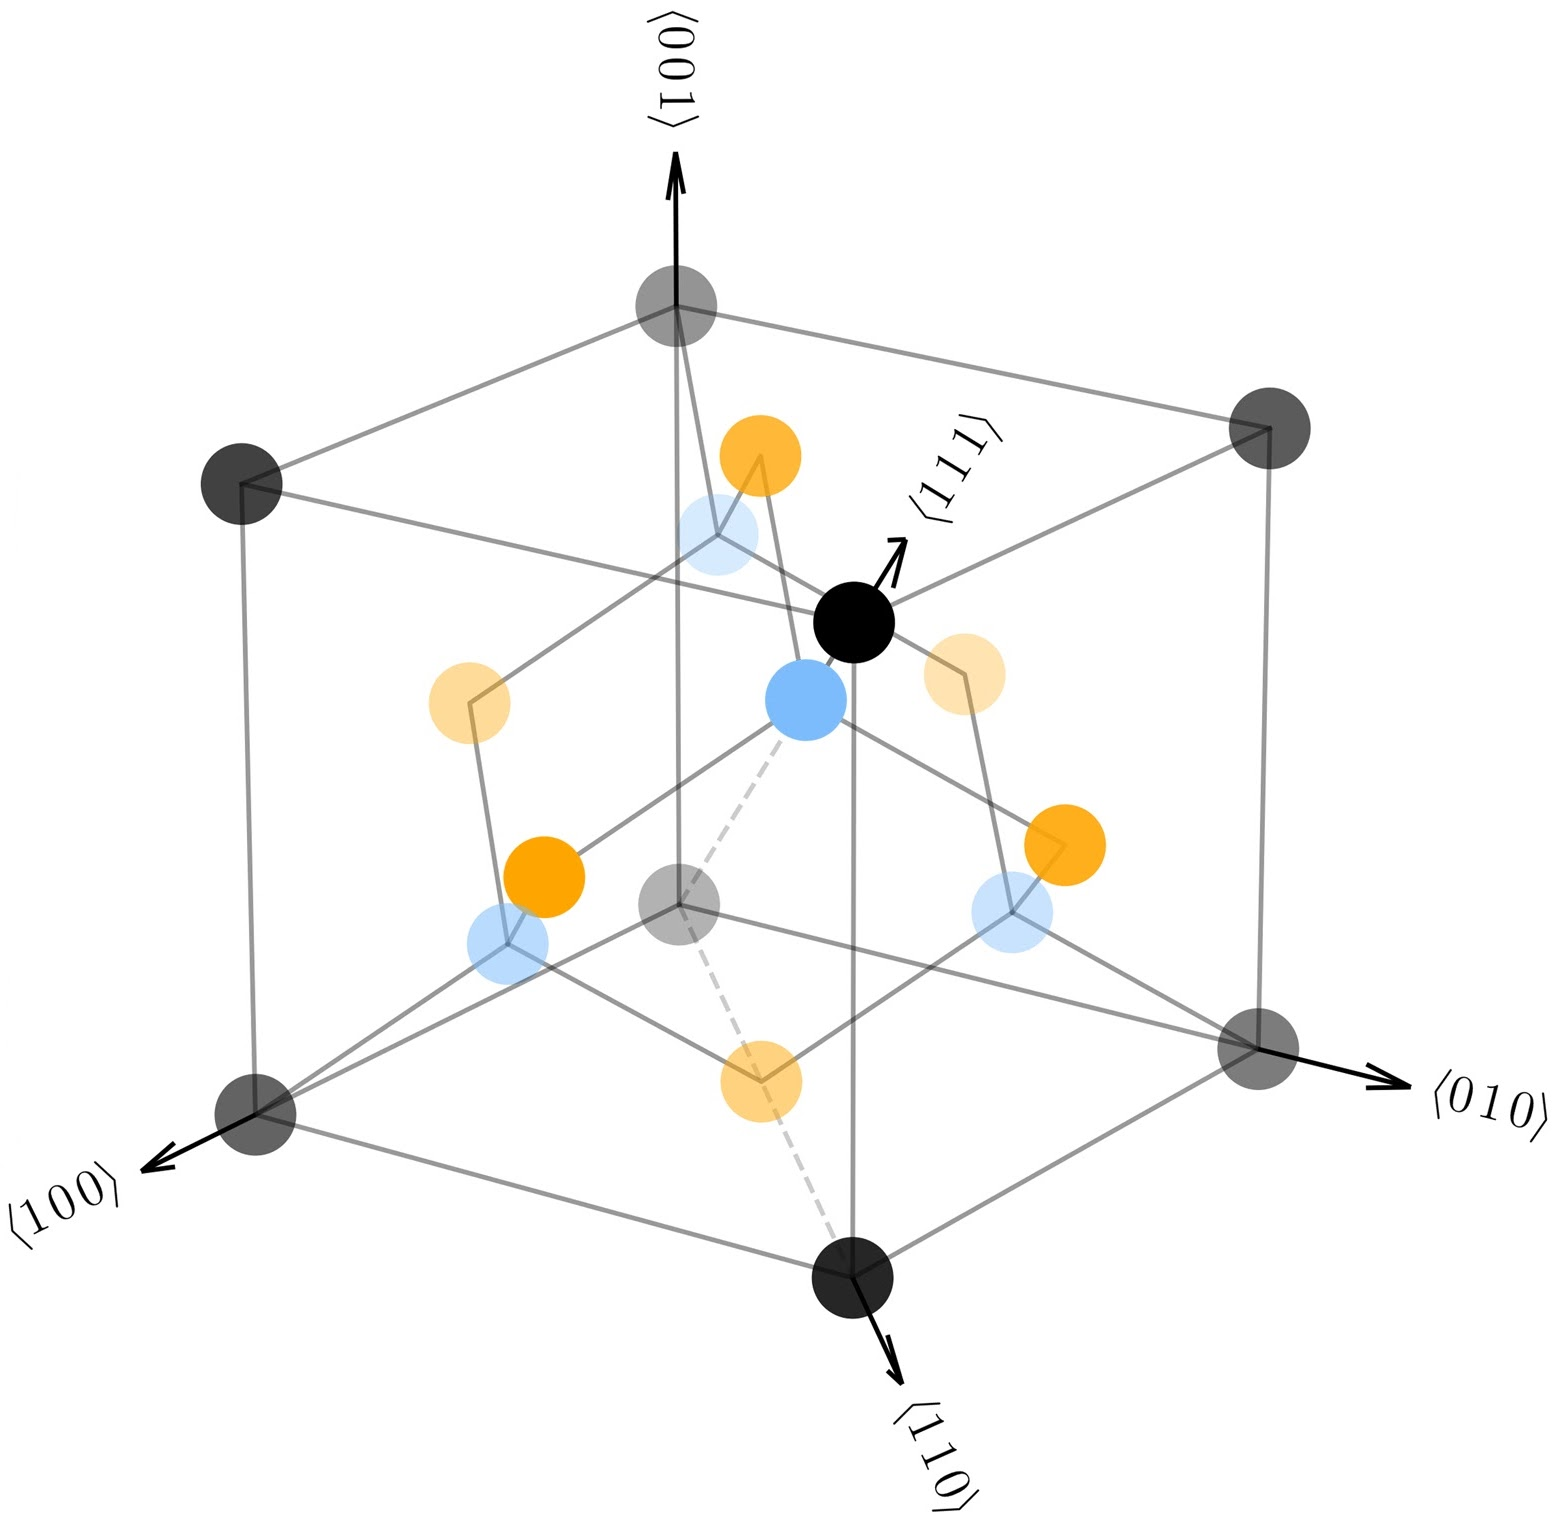
\includegraphics[trim={0cm 0 0cm 0},clip,width=0.6\linewidth]{ch3/figs/ge_crystal_axes.jpg}
    \caption{Germanium crystal unit cell, showing the crystal axis and the crystallographic basis axes. The atoms on the corners, faces and inside the cube are shown in black, orange and blue circles respectively. $\langle 001\rangle$, $\langle 010\rangle$, and $\langle 100\rangle$ are the axes of Ge crystal unit cell. And $\langle 100\rangle$, $\langle 110\rangle$, and $\langle 111\rangle$) are the crystallographic basis axes. The crystallographic basis axes are the direction used to describe physical properties such as mobility and energy band structure. Source: \cite{HervasAguilar2023, Kittel2005}}.
    \label{ch3_figs_ge_crystal_axes}
\end{figure}


\begin{equation}
\vec{v} = \mu_0 \vec{E}
\end{equation}
At higher fields, the scattering with the crystal lattice results in a nonlinear relationship. This scattering causes the velocity to saturate at higher values. The relationship in a higher field can be modeled using \cite{Caughey_1448053}:

\begin{equation}
v(E) = \frac{\mu_0 E}{(1 + (E/E_0)^\beta)^{1/\beta}}
\end{equation}
$\beta$ is the empirical parameter that shapes the curve and typically falls between $0.2$ and $2$.

In {\ehd}, we calculate the electric field in the r and z directions at each point of the grid. We use values from \cite{OMAR19871351}, which gives $v(E)$ from the local electric field $E$. We use a piecewise linear interpolation to find $v(E)$. To do this, we define an array of electric field points, $\texttt{drift\_E}$, which partitions the field range into intervals. For each interval $[E_i, E_{i+1}]$, we store two quantities: a drift offset, corresponding to the drift velocity at $E = E_i$, and a drift slope, which is the rate of change of the drift velocity with respect to the electric field in that interval. The drift velocity is then
computed by:
\begin{equation}
  v(E) \;=\; \text{drift offset}[i]
\;+\; \text{drift slope}[i] \,\bigl( E - E_i \bigr),  
\end{equation}

\noindent
with $E_i \le E < E_{i+1}$. Figure \ref{ch3_fig_dv_vs_e} shows the relation between the drift velocity and the electric field. The drift velocity is then multiplied by the time step to find where the charges will drift, and then the charges are moved to the new location. For simplicity, we only used the $<100>$ direction velocities in the current model. As shown in figure \ref{ch3_fig_dv_vs_e}, for a given electric field magnitude, the variation in mobility with the crystal axis is expected to be $20-40\%$, while the surface drift effects we are studying originate from drift velocities that are up to $1000$ times slower.

\begin{figure}[!htb]
    %[trim={left bottom right top},clip]
    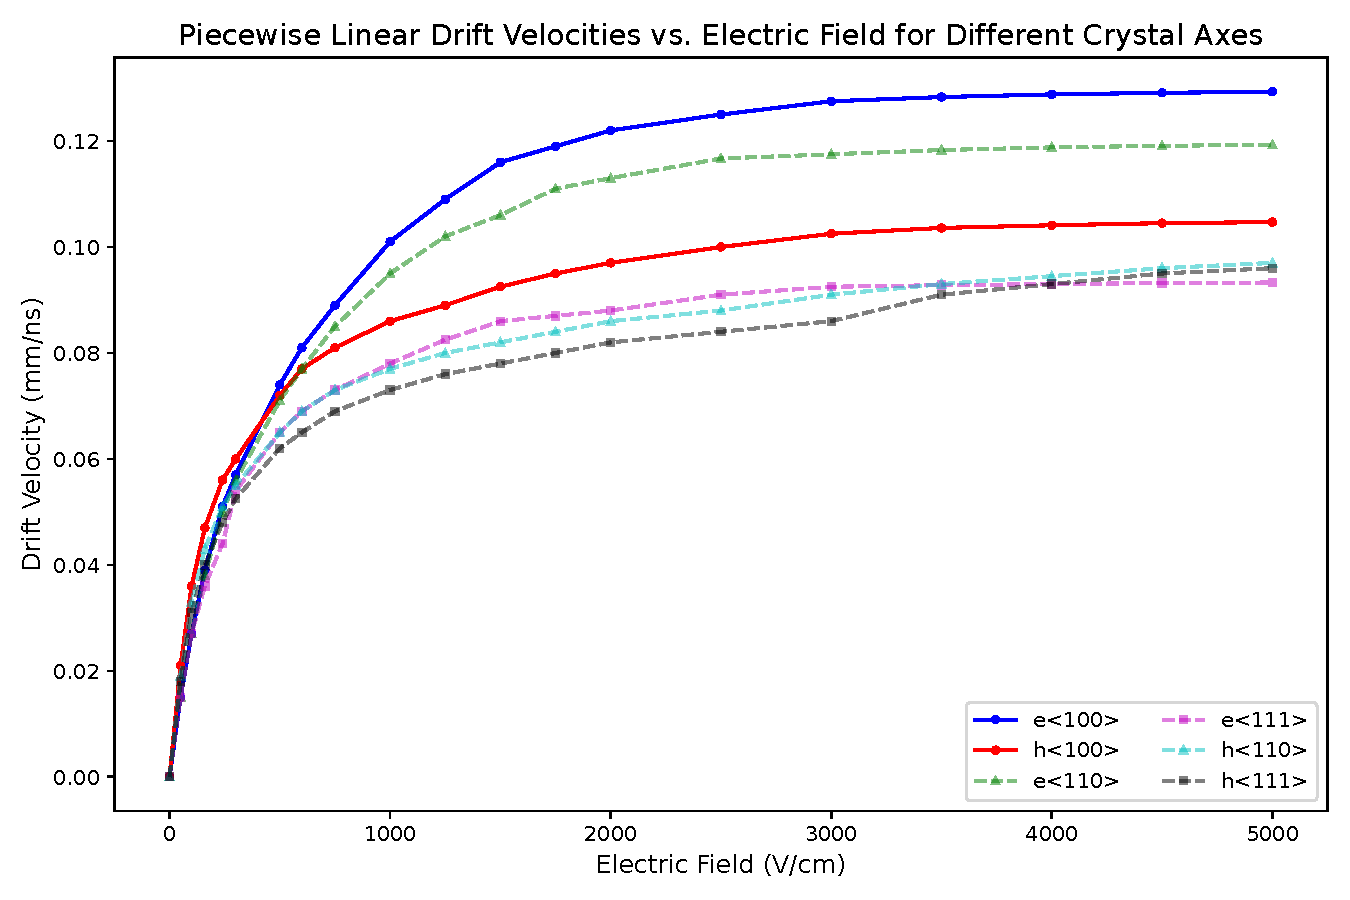
\includegraphics[trim={0cm 0 0cm 0},clip,width=0.99\linewidth]{ch3/figs/ehd_dv_e.pdf}
    \caption{Relation of drift velocity versus electric field in {\ehd}. The points shows the experimental values adapted from \cite{OMAR19871351}. To show how {\ehd} estimates the values we create 500 samples between 0 and 5000 V/cm and performed the piecewise linear interpolation between the points. Only $<100>$ direction velocities are used in the current model.}
    \label{ch3_fig_dv_vs_e}
\end{figure}

\subsubsection*{Fraction Splitting}\label{ch3:sec:frac_split}
We use a splitting approach to move charges to the new cell. Since we are using a grid, we want to account for the discretization by splitting the charges between two grid points. Suppose that after a time step $\Delta t$, the density in the grid cell $(z,r)$ moves $\Delta z$ and $\Delta r$ to a new position $(k,i)$. We use the following equation to define $(k,i)$ and fractional parts $f_z$ and $f_r$:
\begin{align}
k \;=\; z + \Delta z,\quad
f_z \;=\; \lceil \Delta z \rceil - \Delta z\\
i \;=\; r + \Delta r ,\quad
f_r \;=\; \lceil \Delta r \rceil - \Delta r
\end{align}
where $\lceil \Delta z \rceil$ means the floor of z. The charges are split using these fractions:
\begin{align}
&\text{fraction in }(k, i)   \;=\; f_{r} \times f_{z} \\
&\text{fraction in }(k, i+1) \;=\; (1 - f_{r}) \times f_{z}\\
&\text{fraction in }(k+1, i) \;=\; f_{r} \times (1 - f_{z})\\
&\text{fraction in }(k+1, i+1)\;=\; (1 - f_{r}) \times (1 - f_{z}).
\label{eq:bilinear-fractions}
\end{align}
Finally, the densities are updated using:
\begin{align}
\rho^{\mathrm{new}}(k,i)   &\,\mathrel{+}=\, \rho^{\mathrm{old}}(z,r)\times \bigl[f_{r}\times f_{z}\bigr] \times \text{G}_{r,z} \label{ch3:eq:den_update_1} \\
\rho^{\mathrm{new}}(k,i+1) &\,\mathrel{+}=\, \rho^{\mathrm{old}}(z,r)\times \bigl[(1 - f_{r})\,f_{z}\bigr] \times \text{H}_{r,z} \label{ch3:eq:den_update_2} \\
\rho^{\mathrm{new}}(k+1,i) &\,\mathrel{+}=\, \rho^{\mathrm{old}}(z,r)\times \bigl[f_{r}\,(1 - f_{z})\bigr] \times \text{G}_{r,z} \label{ch3:eq:den_update_3} \\
\rho^{\mathrm{new}}(k+1,i+1)&\,\mathrel{+}=\, \rho^{\mathrm{old}}(z,r)\times \bigl[(1 - f_{r})\,(1 - f_{z})\bigr] \times \text{H}_{r,z}. \label{ch3:eq:den_update_4}
\end{align}


\subsection{Geometric Factors}
\label{sec:geom-factor}
In cylindrical coordinates, each cell at index $r$ corresponds to an annular region of approximate circumference $2\pi (r \,\Delta r)$ and thickness $\Delta z$. When the charge moves from cell $(z,r)$ to cell $(k,i)$, we apply the factors:
\[
\text{G}_{r,z} \;\equiv\; \frac{(r-1)}{(i-1)}
\qquad
\text{H}_{r,z} \;\equiv\; \frac{(r-1)}{(i)}
\] 

\noindent
reflecting the difference in volumes at radii $r$ and $i$.
The offsets $(r-1)$ and $(i-1)$ are for one-based indexing in the code. For points near $r=0$ or $i=0$, the code uses a modified factor that preserves volume scaling. 

% The factors \verb|8*r - 8| or \verb|8*i - 8| are specialized scalings to approximate the annular volume near the central axis or near $i=0$. They ensure that even when $r$ or $i$ equals 0 or 1, the total charge remains consistent with the expected geometry. For example, at the very center ($r=0$), a full ring circumference does not exist, so a smaller effective volume must be used. Although such \verb|8*-8| scalings can appear ad~hoc, they are designed to smoothly transition from the central axis to the first few radial rings, thereby avoiding division by zero while preserving charge.

\subsection{Surface Drift}
When charge carriers drift within the detector, they may encounter the passivated surface, which is handled separately. To model the surface, the lowest set of grid points is split into two regions: one modeling the passivated surface of a fixed depth (set by the user and taken by default to be $2\mu$), and one modeling the remaining bulk region, of grid size minus the surface depth. We store the charges on the surface in a special row. 

If the result of the charge drift calculation places a set of charges below the bottom of the detector, they are fully added to the surface row. If the charge enters the passivated layer, we split it up using the fraction splitting used in charge drift. Performing the diffusion on the last grid point in equation \ref{ch3:eq:diffusion_update_2}, the bottom z-point is considered to be the passivated surface. 

We employ the same methods described above for drifting and diffusing the charges present on the surface, but the drift and diffusion are suppressed by the surface drift velocity factor. This factor can be set by the user in a configuration file; it is set to 0.001 by default. It represents the ratio of speed on the surface to that in the bulk and is derived from experimental measurements or computational models of surface drifts. The charges from the surface can drift to the bulk or to other points on the surface. Points on the surface can diffuse to other points on the surface.

\subsection{Courant Number and Adaptive Time Step}
\label{ch3_sec_courant}
The Courant–Friedrichs–Lewy (CFL) condition is a requirement for numerical solutions of partial differential equations involving moving particles \cite{cfl_condition}. It is commonly used in fluid dynamics to ensure that particles travel only to adjacent grid points. We introduce the CFL condition in the {\ehd} to ensure that the time step is well matched to the velocities of the charges. This helps maintain consistency for different input grid sizes. During each simulation time step, we calculate the local Courant number at every point on the grid using the following.

\begin{equation}
C(z,r) = \max \left( \frac{v_r \Delta t}{\Delta x}, \frac{v_z \Delta t}{\Delta x} \right),
\end{equation}

\noindent
where \( v_r \) and \( v_z \) are the drift velocities in r and z directions, respectively, and  \( \Delta x \) is the grid spacing. The time step is updated using the largest Courant number on the grid :
\begin{equation}
\Delta t = \frac{1}{\max (C(z,r))}.
\end{equation}
The use of adaptive time-stepping based on the Courant number minimizes errors from the discretization process while reducing unnecessary computation during periods of the simulation when only slow-moving surface charges are present.

During this calculation, we make an inherent assumption that the drift component in equation \ref{ch3_eq_ehdrift_discrete} has the larger contribution, and thus use it to set the time step. This can be verified by plotting the drift terms ($\mu E_r \rho_r$) and $\mu E_z \rho_z$ against the diffusion terms ($D \nabla \rho_r$ and $D \nabla \rho_z$) as shown in figure \ref{ch3_fig_ehd_pde_comp}. The drift components are an order of magnitude larger than the diffusion components throughout the simulations, which justifies the assumption.


\begin{figure}%[!htb]
    %[trim={left bottom right top},clip]
    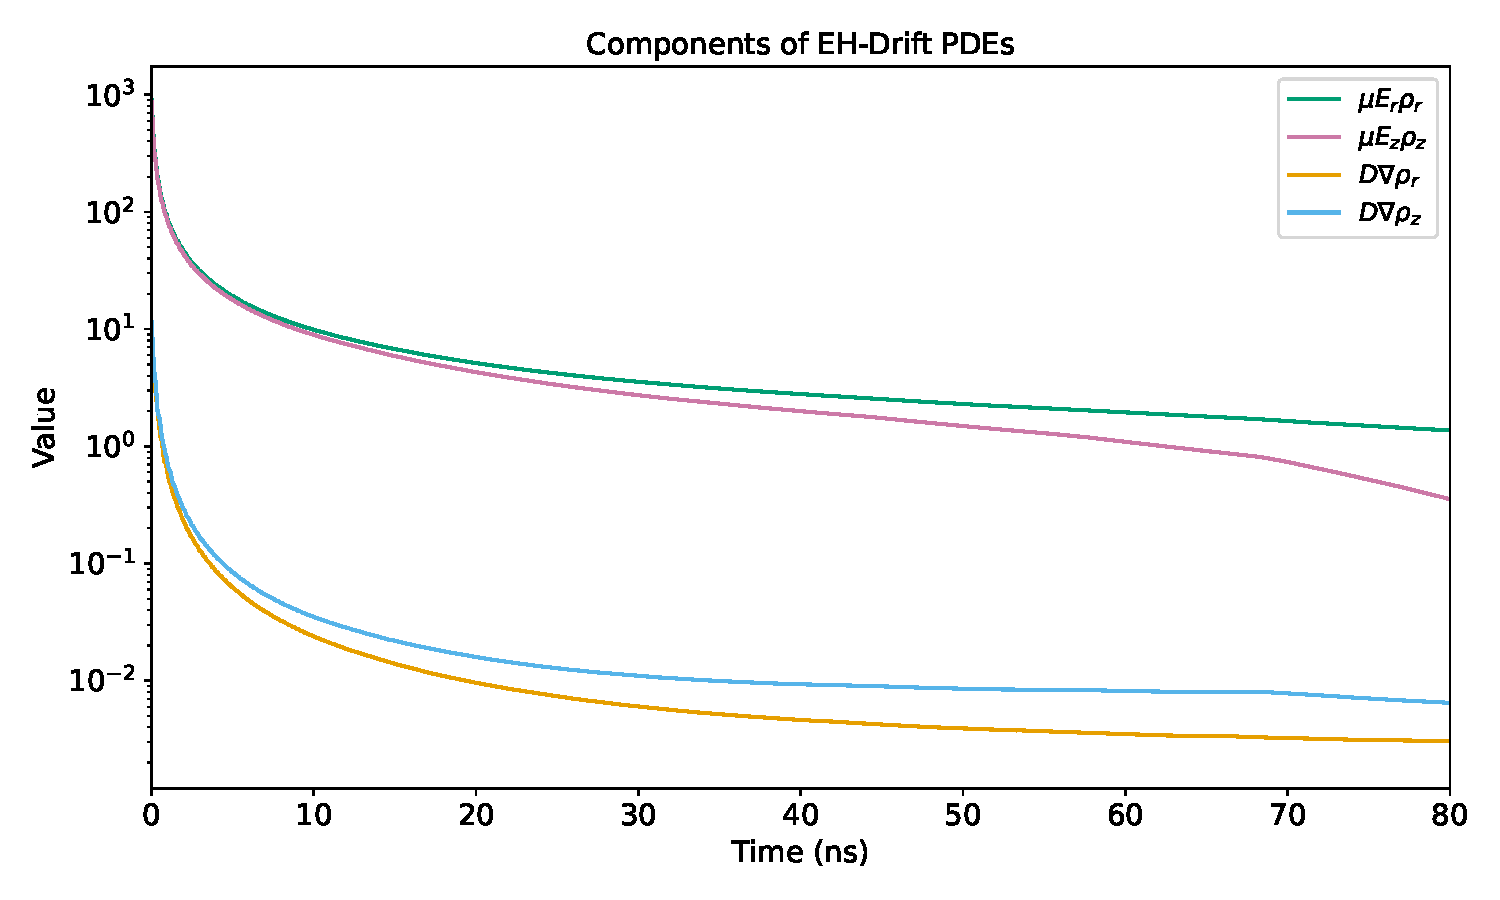
\includegraphics[trim={0cm 0 0cm 0},clip,width=0.99\linewidth]{ch3/figs/ehd_pde_comps.pdf}
    \caption{Maximum values of terms in the charge transport equation \ref{ch3_eq_charge_transport} at a given time step for an event in {\ehd}. The drift terms are about two orders of magnitude large than the diffusion terms throughout the time evolution of the charge cloud. This justifies the use of drift velocity to define the timestep used for Courant number calculation.}    
    \label{ch3_fig_ehd_pde_comp}
\end{figure}


\subsection{Impurity Correction}
Surface events occur in a detector region with low electric fields, and high-energy alpha events, in particular, leave densely ionized tracks. The high density of charge carriers creates a significant local electric field that must be taken into account to accurately calculate the electric potential. At a given time, the impurity correction is given by:

\begin{equation}
  {\text{I}_{t}}(z, r) = \text{I}_{0}(z, r) +
  \bigl( \rho_h(z, r) - \rho_e(z, r) \bigr) \times \frac{e}{\epsilon} \times \frac{(\Delta x)^2}{2}.
\end{equation}

\noindent
The $\text{I}_{0}$ is the bulk impurity level of the crystal, measured at production. $\rho_h(z,r)$ and $\rho_e(z,r)$ are the hole and electron densities, respectively. $\frac{e}{\epsilon}$ is the conversion factor that relates the charge density to the resulting electric field, derived from Gauss's law in Germanium with $\epsilon = 16\epsilon_0$. $\frac{e}{\epsilon}$ is $11.310$ in
charge units of $10^{10}\frac{e}{cm^3}$. $(\Delta x)^2$ is the area of the grid that converts the density to charge, and then the conversion factor converts it into $10^{10}\frac{e}{cm^3}$ units to match the units of impurity used.

\subsection{Signal Calculation}
In cylindrical coordinates, each grid cell with radius $r$ and height $z$ has an area proportional to $(r - 1)$. Once we read the electron density $\rho_e(r,z)$ and hole density $\rho_h(r,z)$ at time $t$, the weighted sums are defined as:

\begin{align}
S_e(t) \;=\; \sum_{z=1}^{L-1} \sum_{r=1}^{R-1}
   \rho_e(r,z)\,\bigl(r-1\bigr)\,\text{wpot}[r-1][z-1]\\
S_h(t) \;=\; \sum_{z=1}^{L-1} \sum_{r=1}^{R-1}
   \rho_h(r,z)\,\bigl(r-1\bigr)\,\text{wpot}[r-1][z-1],
\end{align}

\noindent
where \(\texttt{wpot}[\,r-1\,][\,z-1\,]\) is the weighting potential at that point in the grid. These $S_e(t)$ and $S_h(t)$ represent the induced signal contributions of electrons and holes, respectively, using the Shockley-Ramo theorem.

The initial unweighted sums are defined as:
\begin{align}
R_{e}(0) \;=\; \sum_{z=1}^{L-1} \sum_{r=1}^{R-1}
   \rho_e(r,z)\,\bigl(r-1\bigr), \quad \\
R_{h}(0) \;=\; \sum_{z=1}^{L-1} \sum_{r=1}^{R-1}
   \rho_h(r,z)\,\bigl(r-1\bigr), \quad
\end{align}
% They keep track of how many electrons or holes remain in the crystal at time $t$ 
% (as opposed to how much they contribute to the signal).  For instance, if 
% $R_{h}(t)$ drops below $R_{h}(0)$, that implies some fraction of holes 
% has reached the collecting electrode or left the active region.
\noindent
Combining these quantities, the induced signal at time t is computed using:
\begin{equation}
\text{Signal}[\,t\,] 
\;=\;
  \frac{\,S_h(t)\;-\;S_h(0)\,}{\,R_{h}(0)\,}
  \;-\;
  \frac{\,S_e(t)\;-\;S_e(0)\,}{\,R_{e}(0)\,}
\label{eq:net-signal}
\end{equation}

\noindent
Since the electrons' contribution would be negative, we subtract it from holes to get the net induced signal. Normalization by $R_{e}(0)$ and $R_{h}(0)$ ensures that the signal is expressed as a fraction of the original total electron/hole count, so it starts near zero at $t=0$ and approaches 1 as all charges arrive at the contacts.

\subsection{Density Snapshots}
The ability to store density snapshots at each time step provides detailed information about how the charges drift in the detector. Figure \ref{ch3_fig_ehd_path_pd_sc_0} shows a snapshot at time=$80$ns in an {\ehd} simulation for a 5 MeV energy deposition close to the surface without any surface charge. The event started at r=15 mm. The electrons drift towards the n$^+$ contact, which is located to the right at $r=34.7$mm, and the holes drift towards the p$^+$ contact, located to the left starting at $r=1.5$mm. A 5 MeV energy deposition can create a charge cloud 1.5 mm high. Charges in such a large charge cloud drift and diffuse to the surface, even in the absence of surface charges. The projected density (bottom panel of figure \ref{ch3_fig_ehd_path_pd_sc_0}) shows the density of the charge cloud as a function of radius. The peak of each distribution is created by the charges traveling normally through the bulk of the detector. The broad tail of the projected density has an additional secondary peak, seen at r = 15 mm, which is due to the charges that were initially pushed to the surface by self-repulsion when the charge clouds were at their highest density. The points in between the two peaks are charges that drifted or diffused to the surface in intermediate steps. 

\begin{figure}%[!htb]
    %[trim={left bottom right top},clip]
    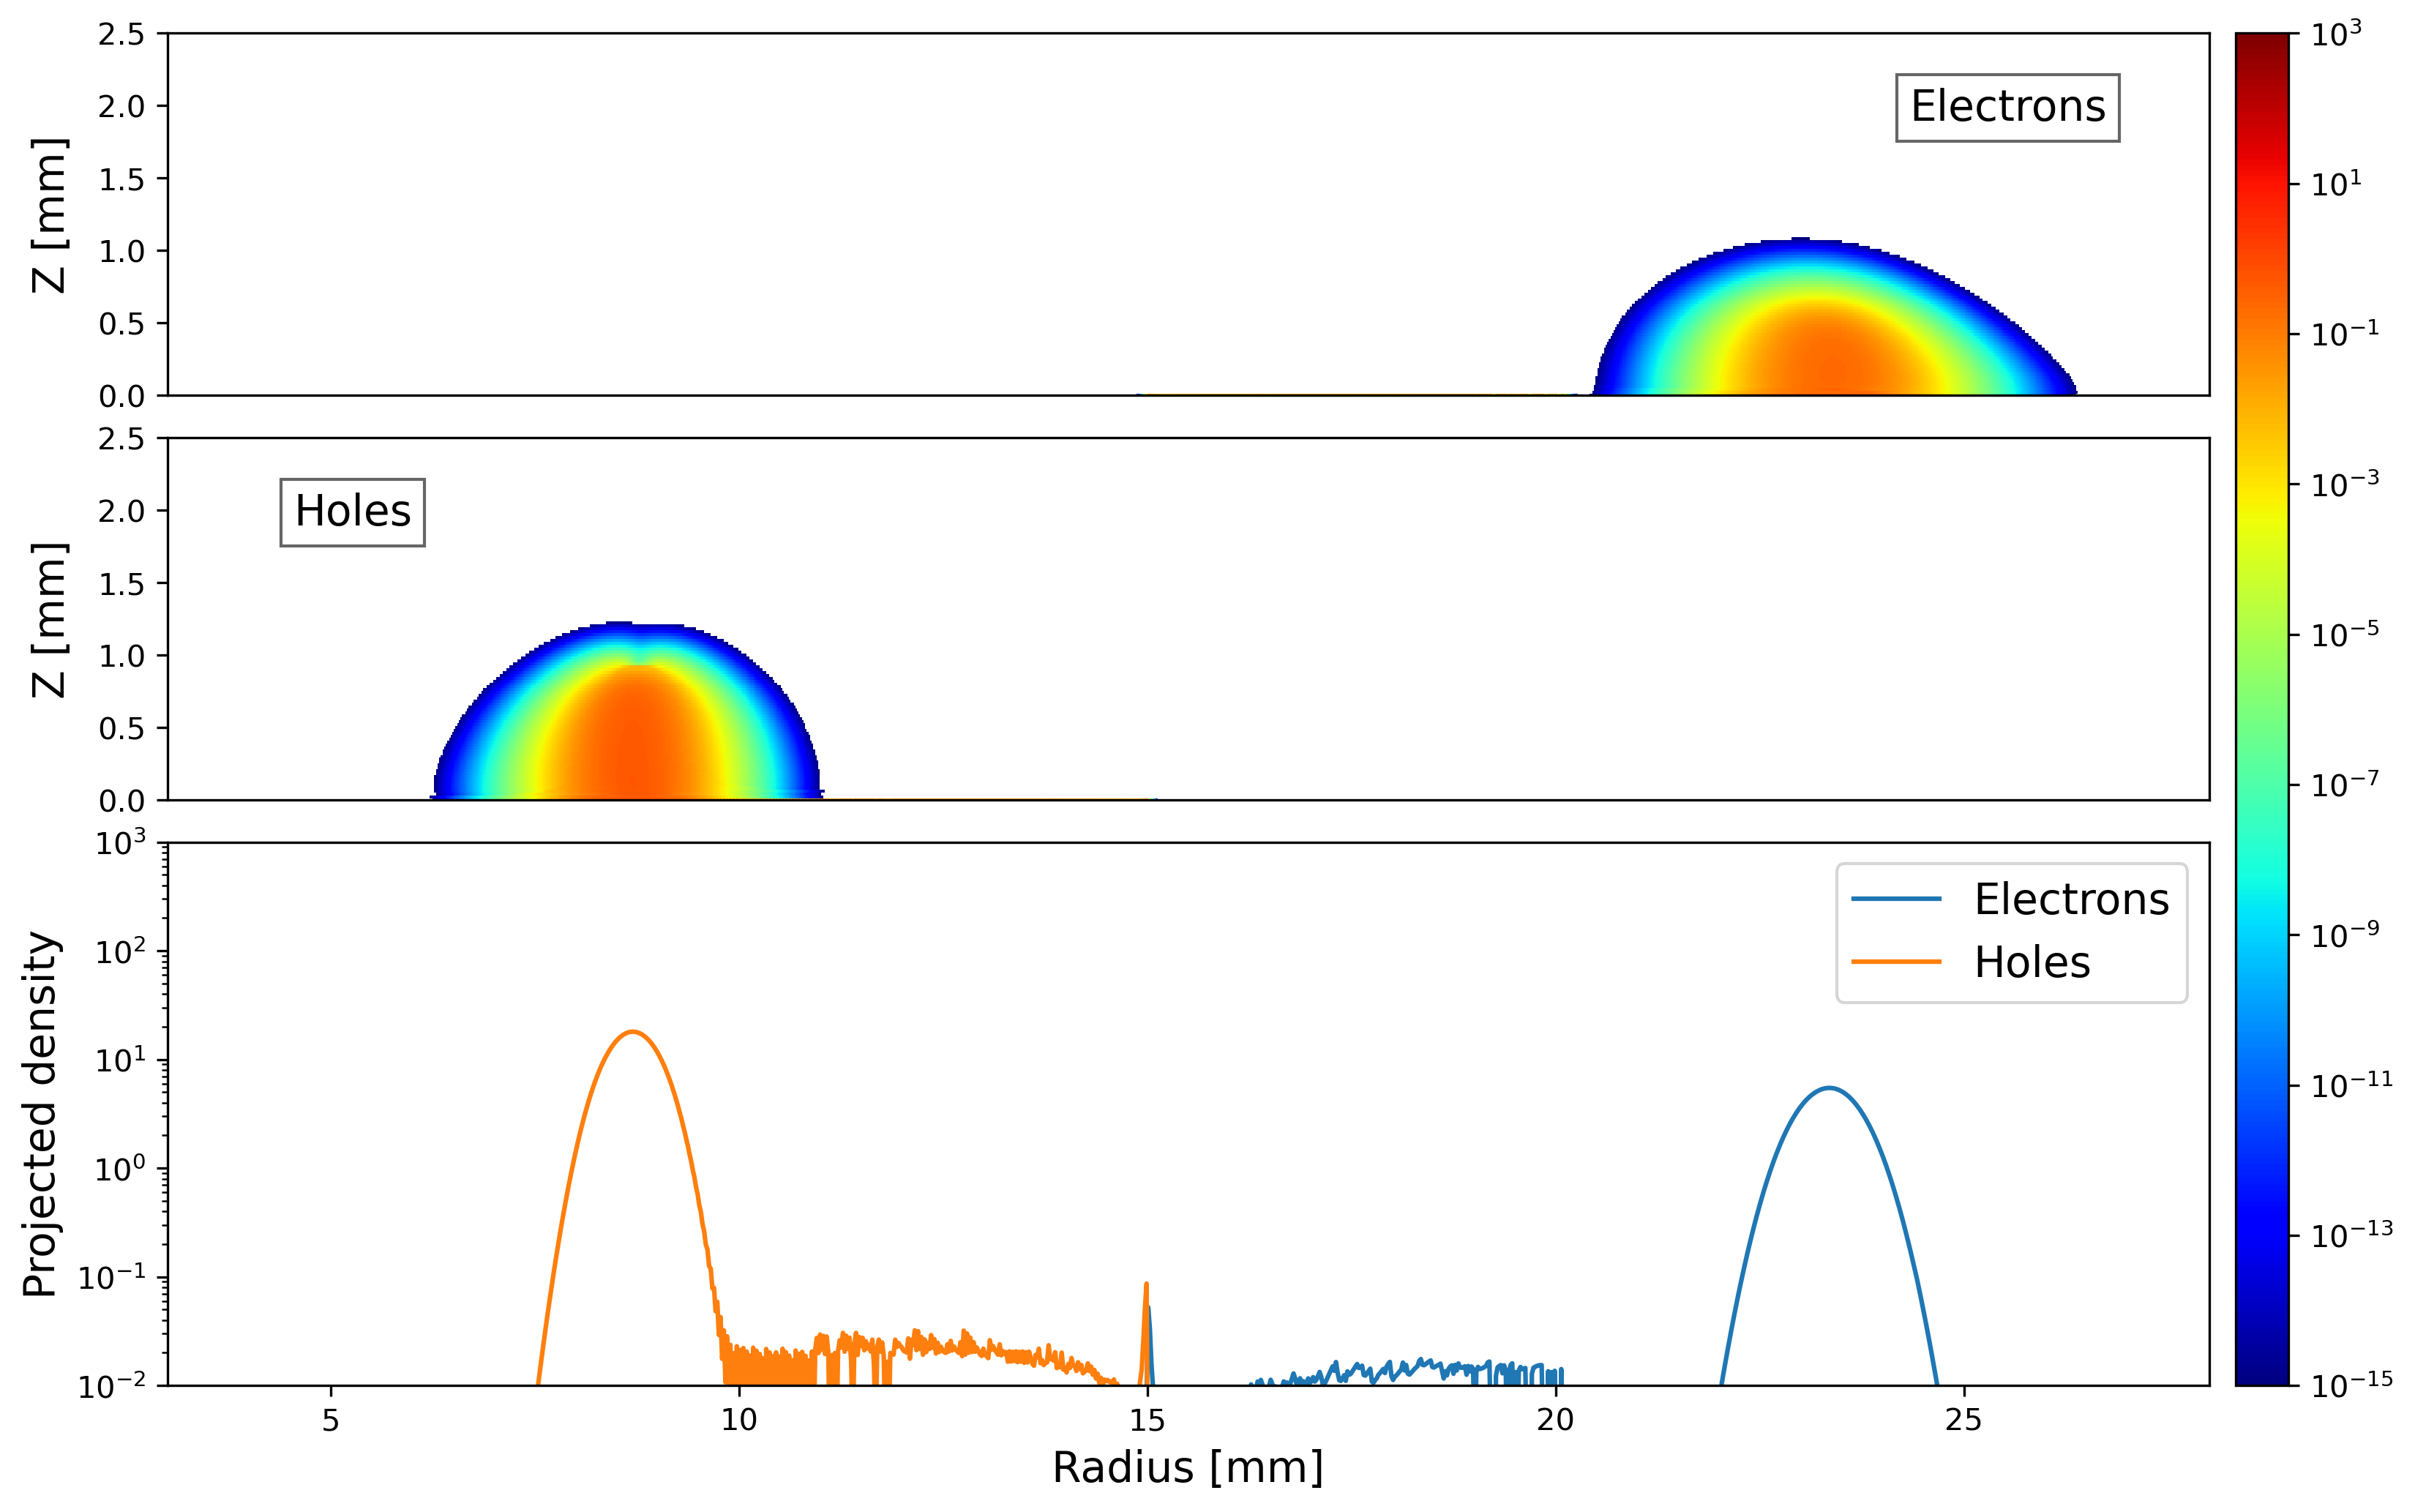
\includegraphics[trim={0cm 0 0cm 0},clip,width=0.99\linewidth]{ch3/figs/drift_path_sc=0.0.png}
    \caption{Drift of electron and hole charge clouds in {\ehd} with zero surface charge. The projected densities show how the charges are distributed along the radius. The densities have two peaks, one due to the fast moving component in bulk and another due to the slow moving component on the passivated surface.}
    \label{ch3_fig_ehd_path_pd_sc_0}
\end{figure}

Figure \ref{ch3_fig_ehd_path_pd_sc_neg_0p3} shows the same event at the same time, but with a negative charge on the surface. The negative charges alter the field in such a way that holes are pulled onto the surface and electrons are repelled. Thus, the holes have a significant fraction of their charge attracted to the surface, as seen in the projected density plot. Electrons, being repelled from the surface, have no slow-moving component.


\begin{figure}%[!htb]
    %[trim={left bottom right top},clip]
    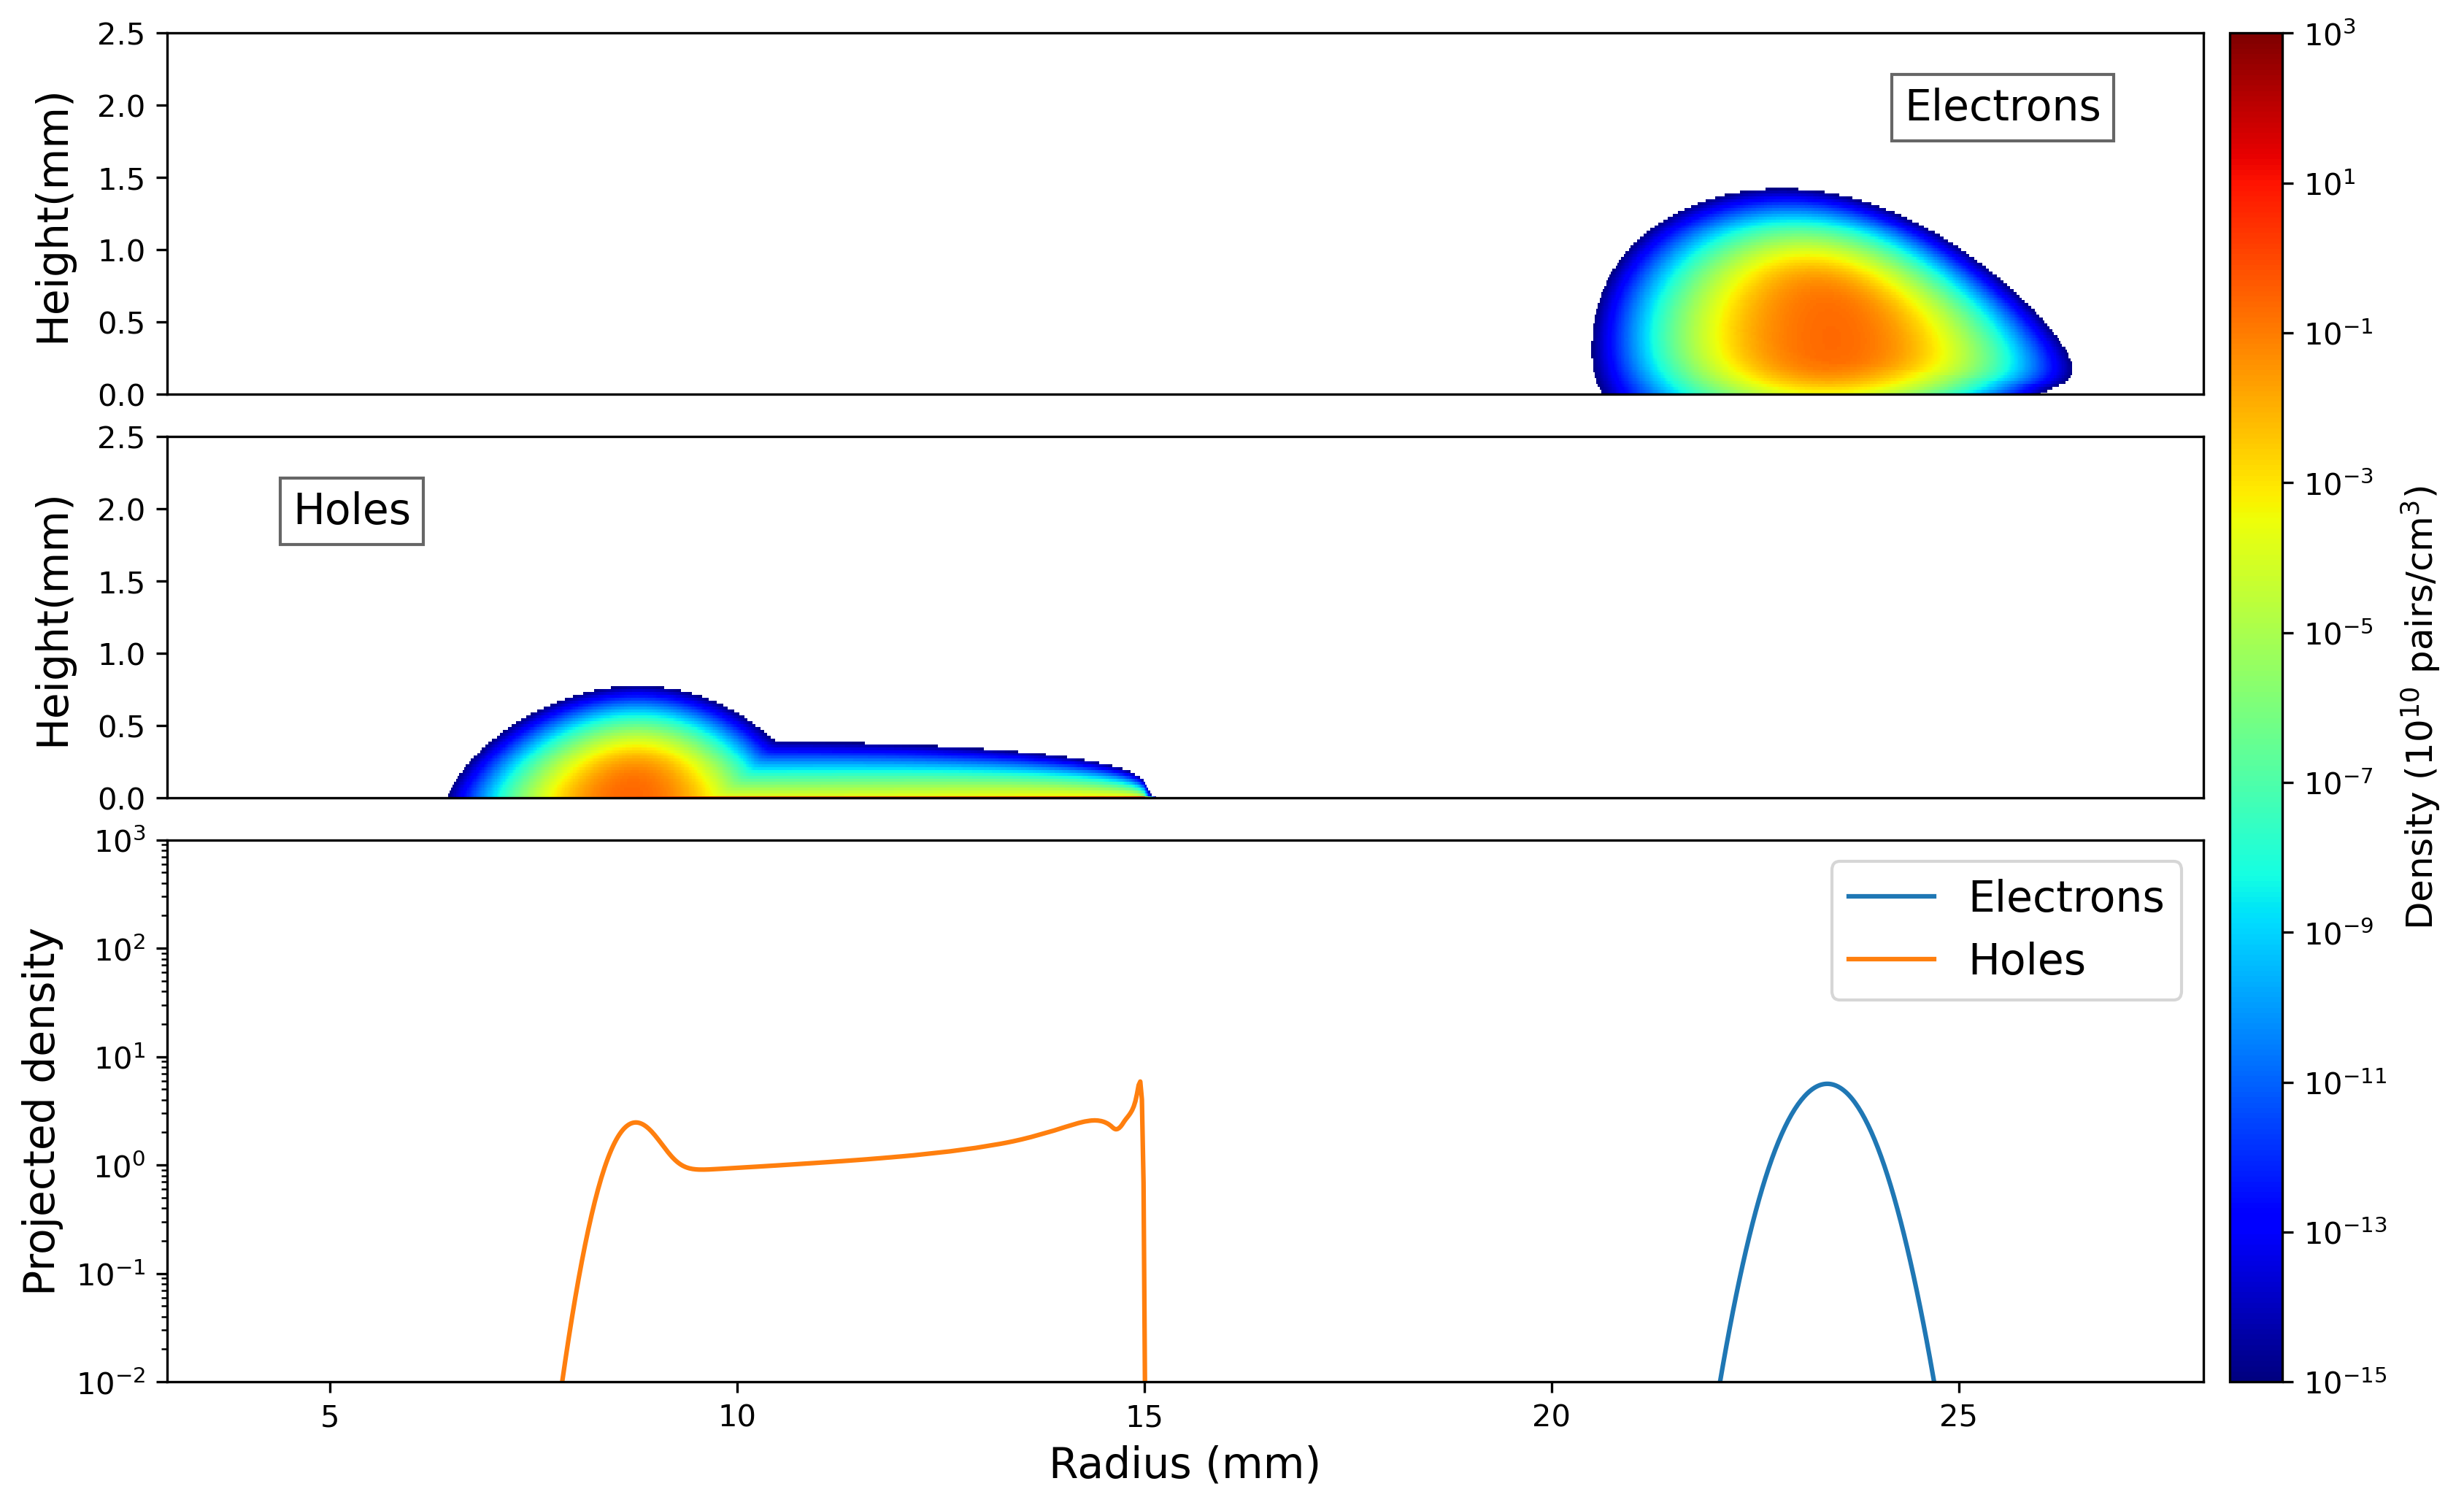
\includegraphics[trim={0cm 0 0cm 0},clip,width=0.99\linewidth]{ch3/figs/drift_path_sc=-0.3.png}
    \caption{Drift of electron and hole charge clouds in {\ehd} with negative surface charge. The negative surface charge pulls the holes onto the surface, which then move at a slower speed.}
    \label{ch3_fig_ehd_path_pd_sc_neg_0p3}
\end{figure}

Similarly, Figure \ref{ch3_fig_ehd_path_pd_sc_pos_0p3} shows the same event but with a positive charge on the surface. In this case, the electrons are pulled onto the surface and drift slowly, while the holes are repelled and do not have surface drift. 

\begin{figure}%[!htb]
    %[trim={left bottom right top},clip]
    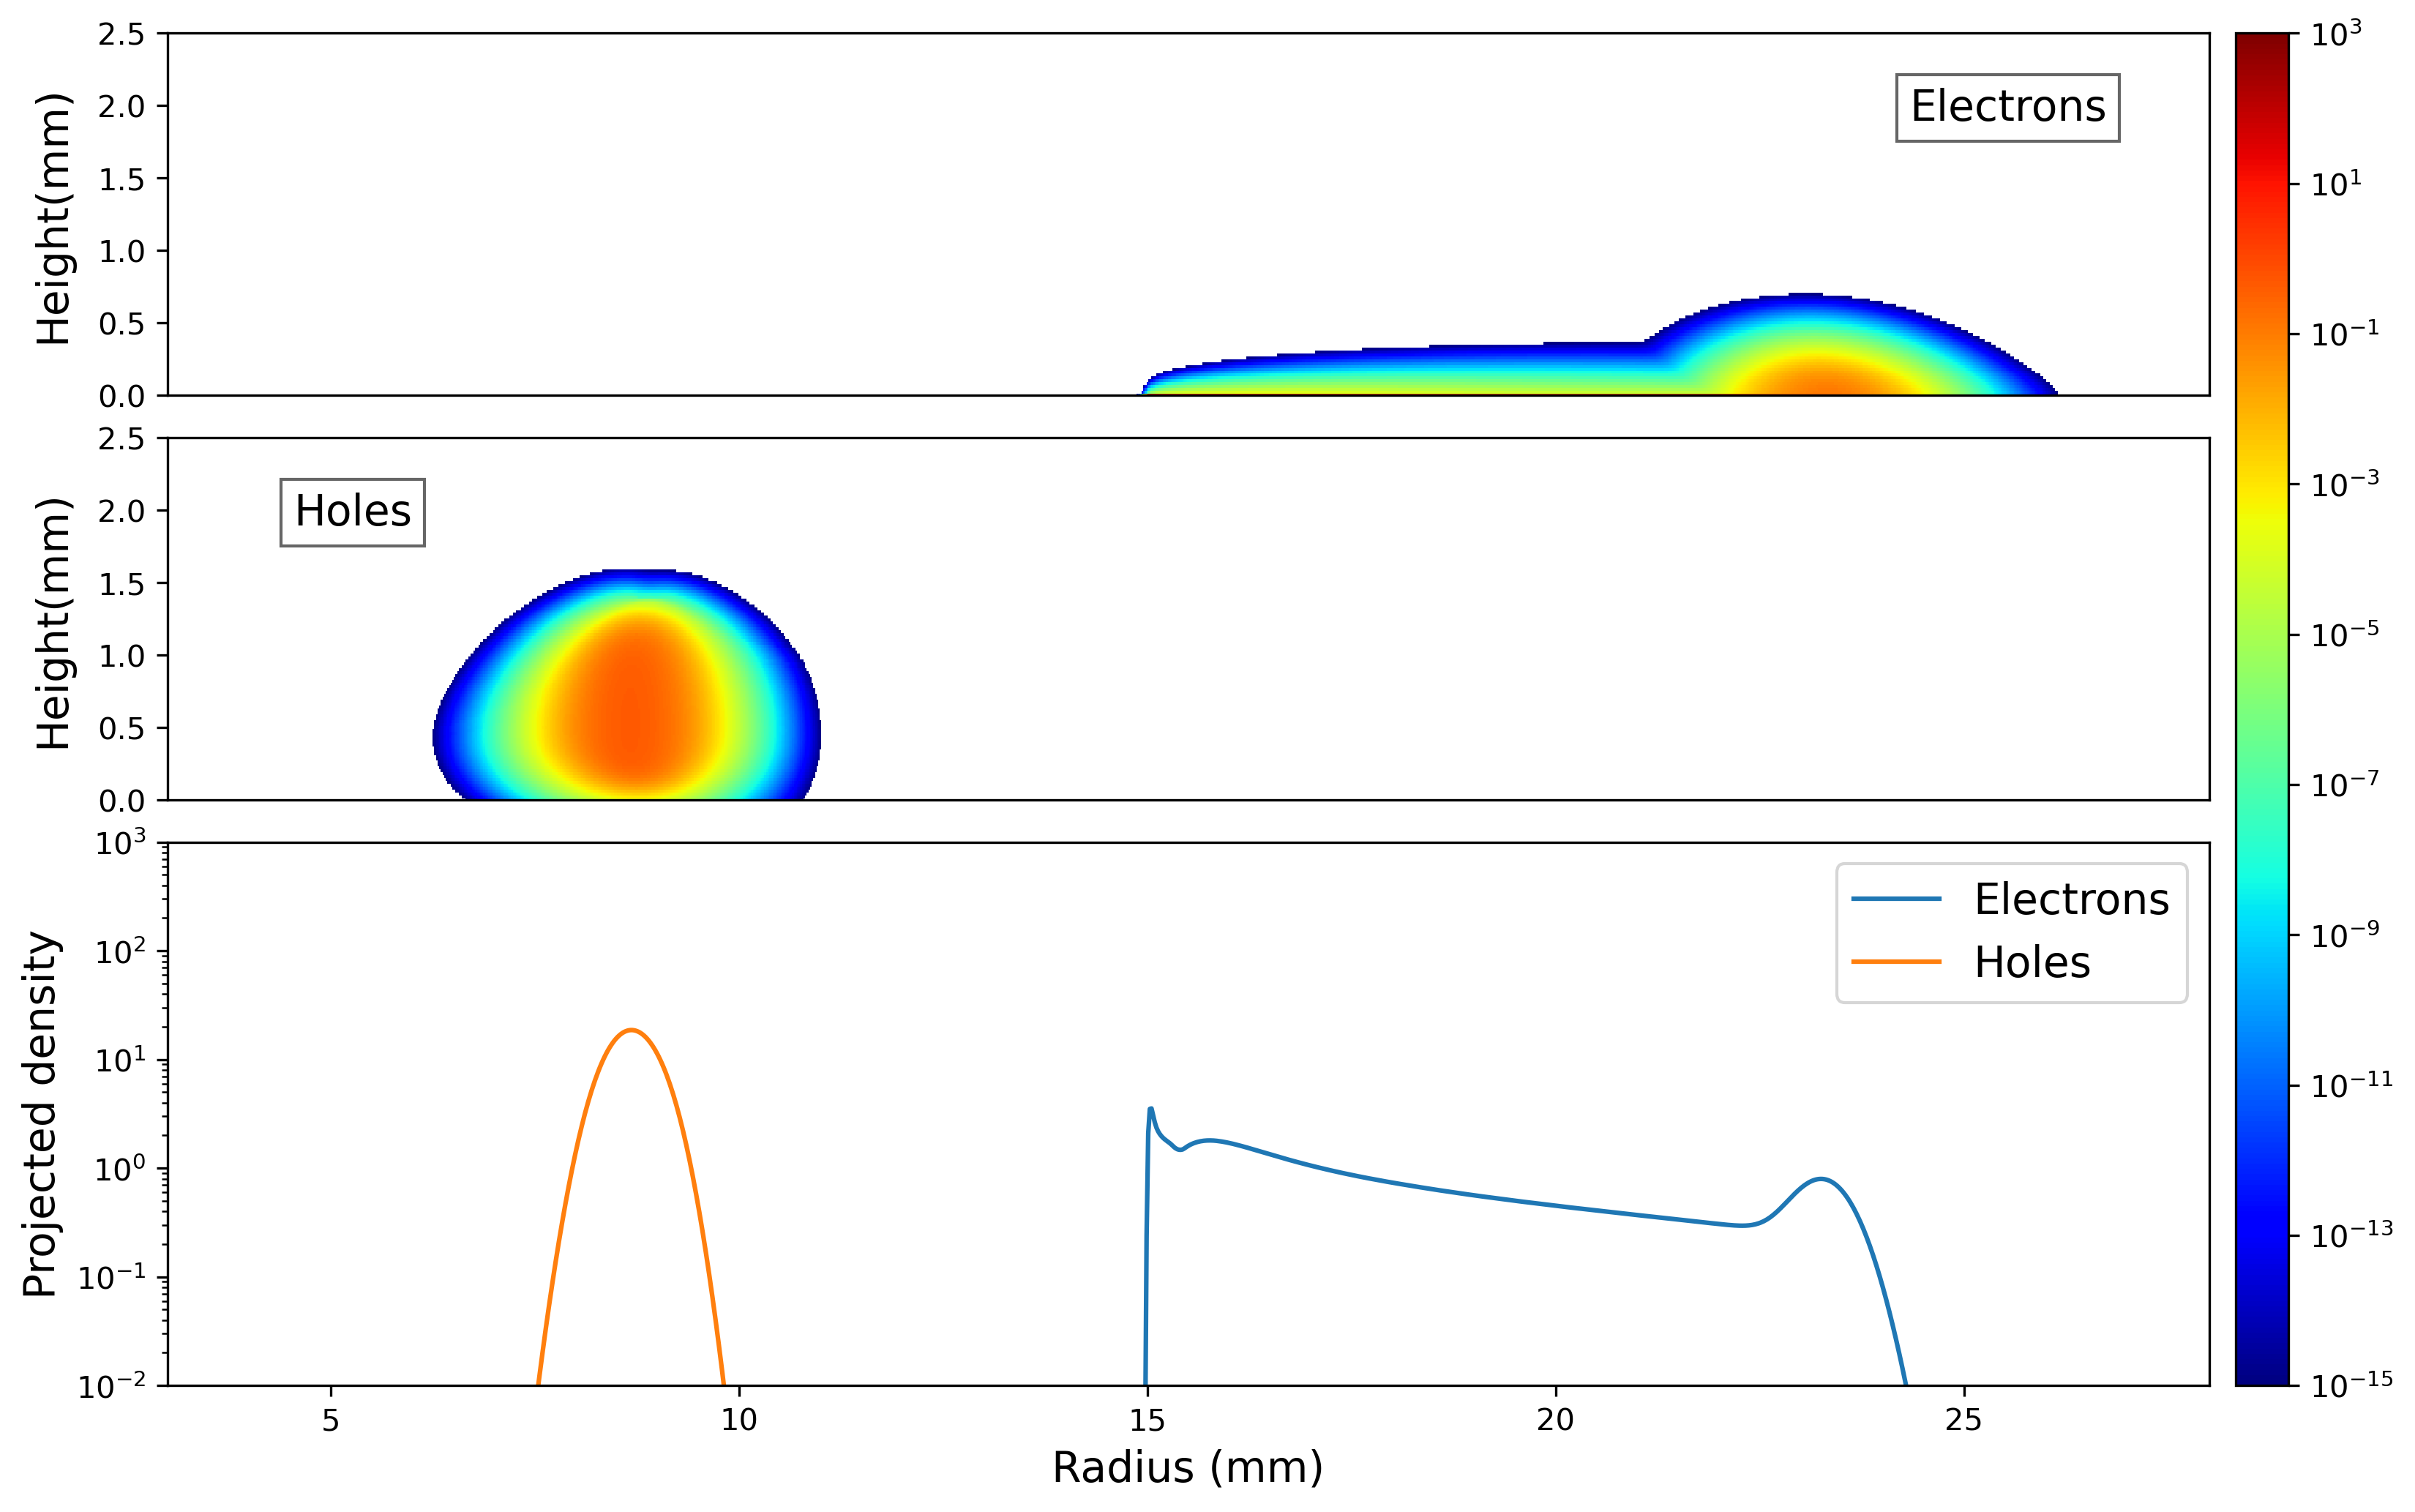
\includegraphics[trim={0cm 0 0cm 0},clip,width=0.99\linewidth]{ch3/figs/drift_path_sc=0.3.png}
    \caption{Drift of electron and hole charge clouds in {\ehd} with positive surface charge. The positive surface charge pulls the electrons onto the surface which move at a slower speed.}
    \label{ch3_fig_ehd_path_pd_sc_pos_0p3}
\end{figure}


\subsection{Model Parameters}
In {\ehd}, certain inputs can be adjusted to match the observed data. These parameters fall into three categories: event-to-event quantities, detector-level constants, and operating conditions.

Event-to-event quantities such as the initial energy and event position are known or fixed by the source configuration, such as a mono-energetic alpha beam or a background location from Monte Carlo simulations. These would not usually vary to match data, but rather set based on the known test stand or source energy.

Detector-level constants, such as passivated surface thickness or the ratio of surface-to-bulk drift speed, are physically determined by the detector fabrication and inherent surface conditions. Although these remain constant for a single detector, they may not be well measured and thus serve as unknown but fixed parameters. Tuning them helps reproduce the shape of waveforms. Figure \ref{fig:wf_comp} illustrates how the shape of the resulting waveform changes as surface-to-bulk drift and surface charge vary. The high magnitude of the surface charge means that more charges will be pulled onto the surface, and thus the sharply rising part of the waveform, which is due to bulk charge collection, will have a lower magnitude. A faster surface-to-bulk ratio means that the charges on the surface will be collected more quickly, and therefore the tail shape will be different.

The deployment or operating conditions, such as surface charge density or bias voltage, can change between different experimental setups or over time. The surface charge, for instance, might build up differently after each deployment, while the operating voltage is controlled by the detector configuration and the conditions of the experiment.

\begin{figure}%[!htb]
    %[trim={left bottom right top},clip]
    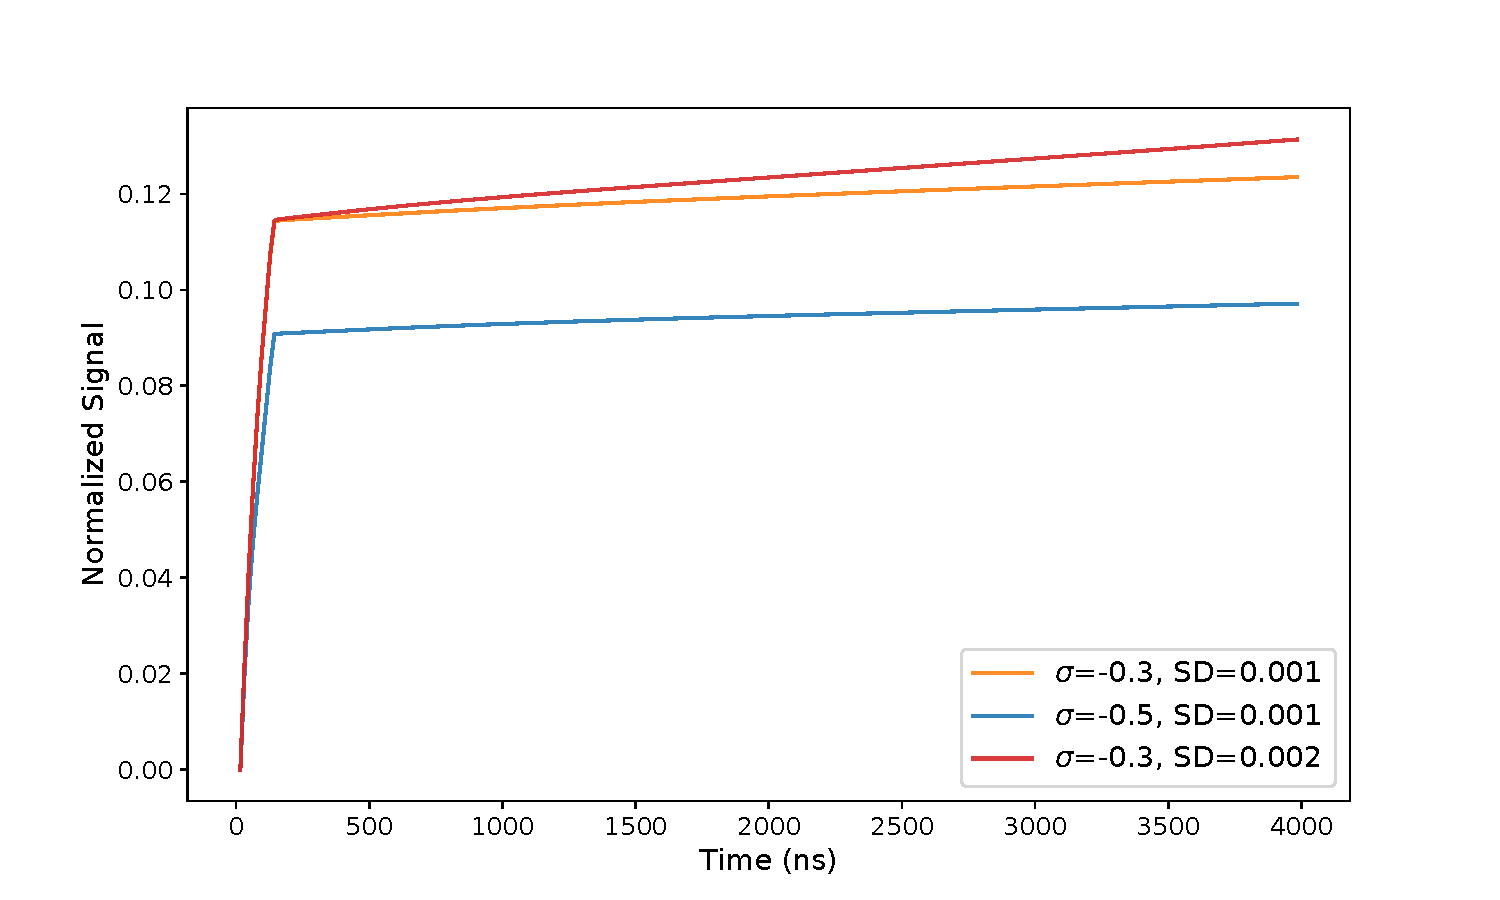
\includegraphics[trim={0.1cm 0.3cm 1.3cm 0.3cm},clip,width=0.99\linewidth]{ch3/figs/wf_comp.pdf}
    \caption{A comparison of waveforms generated by {\ehd} for a {\Ltwo} PPC detector as surface charge ($\sigma$) and relative surface drift velocity (SD) are varied. The events were at r=15 mm z=0.02 mm.}
    \label{fig:wf_comp}
\end{figure}


\subsection{Input and Output}
{\ehd} is compiled using the GCC compiler. It utilizes a configuration file that is the same as {\siggen}. The configuration file contains information on the detector geometry, and an example can be found in \cite{ehdrift2024}. In addition to the configuration file, we provide flags that can be passed to the executable. Table \ref{ch3_tab_ehdrift_parameters} shows the input flags that allow one to set multiple parameters related to the event.
\begin{table}[!htb]
    \centering
    \renewcommand{\arraystretch}{1.3} % Adjust row spacing
    \begin{tabular}{|l|p{10cm}|c|}
        \hline
        \textbf{Flag} & \textbf{Description} & \textbf{Example} \\ 
        \hline
        -r & Set the radial position of the event in mm. & 15.00 \\
        \hline
        -z & Set the axial position of the event in mm. & 0.50 \\
        \hline
        -g & Specify the detector name. & P42575A \\
        \hline
        -s & Set the surface charge density in $10^{10} e/\text{cm}^2$. & -0.50 \\
        \hline
        -e & Input the interaction energy in keV. & 5000 \\
        \hline
        -v & Choose whether to write density files (0 = no, 1 = yes). & 1 \\
        \hline
        -f & Choose whether to recalculate the electric field (0 = no, 1 = yes). & 1 \\
        \hline
        -w & Choose whether to save the electric field (0 = no, 1 = yes). & 1 \\
        \hline
        -d & Choose whether to save the depletion surface (0 = no, 1 = yes). & 1 \\
        \hline
        -p & Choose whether to write the weighting potential (0 = no, 1 = yes). & 1 \\
        \hline
        -b & Set the bias voltage in volts. & 3500 \\
        \hline
        -h & Specify the grid size in mm. & 0.0200 \\
        \hline
        -m & Define the passivated surface depth in mm. & 0.10 \\
        \hline
        -c & Set the velocity of surface charges compared to bulk. & 0.75 \\
        \hline
        -a & Input a custom impurity density profile file. & filename.dat \\
        \hline
        -t & Define the total simulation run time in ns. & 16000 \\
        \hline
        -u & Set the frequency of output signal saving in ns. & 16 \\
        \hline
    \end{tabular}
    \caption{Input parameters to EH-Drift}
    \label{tab:ehdrift_parameters}
\end{table}



The simulation output is stored in an HDF5 file, a hierarchical data format optimized for handling large structured datasets. Each simulated event is recorded in the `event data' dataset as a compound data type containing energy, radius and height positions, surface charge, surface drift velocity factor, and the signal for the event. The dataset is dynamically extendable to allow new events to be appended without rewriting existing data. The file includes grid size, passivated surface thickness, self-repulsion flag, and detector name as attributes. Attributes are stored as scalars at the file root level for efficient retrieval without redundancy. This storage is critical for High Performance Computing (HPC) when we simulate thousands of waveforms for multiple detectors.